\documentclass[11pt,a4paper]{article}

% ============================================================
%  PACKAGES
% ============================================================
\usepackage[utf8]{inputenc}
\usepackage[T1]{fontenc}
\usepackage[margin=2.5cm]{geometry}
\usepackage{graphicx}
\usepackage{booktabs}
\usepackage{amsmath}
\usepackage{amssymb}
\usepackage{xcolor}
\usepackage{caption}
\usepackage{float}
\usepackage{array}
\usepackage{multirow}
\usepackage{enumitem}
\usepackage{fancyhdr}
\usepackage{setspace}
\usepackage[colorlinks=true, linkcolor=blue!50!black, citecolor=blue!50!black,
urlcolor=blue!50!black, linktoc=all]{hyperref}

% ============================================================
%  GENERAL SETTINGS
% ============================================================
\setstretch{1.08}
\setlength{\emergencystretch}{3em}
\captionsetup{font=small, labelfont=bf, margin=10pt}
\renewcommand{\arraystretch}{1.15}

\pagestyle{fancy}
\fancyhf{}
\fancyhead[L]{\small EEG Motor Imagery Classification -- Project Report}
\fancyhead[R]{\small \thepage}
\renewcommand{\headrulewidth}{0.4pt}

\newcommand{\acc}{\text{Acc}}
\newcolumntype{C}[1]{>{\centering\arraybackslash}p{#1}}

% ============================================================
%  TITLE PAGE
% ============================================================
\title{
	\vspace{-1.5cm}
	{\large BCI Competition IV-2a: A Comparative Study}\\[0.4cm]
	\rule{\linewidth}{0.5pt}\\[0.3cm]
	{\Huge \bfseries Cross-Subject Generalization in EEG-Based \\[0.2cm] Motor Imagery Classification}\\[0.3cm]
	\rule{\linewidth}{0.5pt}\\[0.4cm]
	{\large Subject-Dependent Baselines, Leave-One-Subject-Out Cross-Validation, \\
		and Deep Learning (EEGNet) Approaches}
}

\author{
	Author Name \\
	\small Department of \emph{[Your Department]}, \emph{[Your University]} \\
	\small \texttt{[your.email@university.edu]}
}

\date{\today}

% ============================================================
%  DOCUMENT
% ============================================================
\begin{document}
	
	\maketitle
	\thispagestyle{empty}
	
	\begin{abstract}
		\noindent
		Brain--Computer Interfaces (BCIs) based on motor imagery (MI) electroencephalography (EEG) promise
		non-invasive control pathways for assistive and rehabilitation technology, but their real-world
		deployment is hindered by pronounced inter-subject variability in EEG signal statistics. This report
		presents a comparative experimental study of three modelling strategies applied to the nine-subject
		BCI Competition IV-2a motor-imagery dataset (left hand, right hand, feet, tongue). First, a hybrid
		feature-engineering pipeline combining Wavelet Packet Decomposition (WPD), Filter-Bank Common Spatial
		Patterns (CSP), and a Multi-Layer Perceptron (MLP) classifier is trained exclusively on a single
		subject and evaluated on the remaining eight, revealing a severe cross-subject generalization gap
		(in-sample accuracy $0.759$ vs.\ mean unseen-subject accuracy $0.317 \pm 0.074$, chance $=0.250$).
		Second, the same hybrid pipeline is re-evaluated under a Leave-One-Subject-Out (LOSO) cross-validation
		protocol across all nine subjects, incorporating Euclidean-Alignment covariance whitening, which
		raises the mean cross-subject accuracy modestly to $0.401 \pm 0.125$. Third, EEGNet, a compact
		convolutional neural network purpose-built for EEG decoding, is trained end-to-end under the same
		LOSO protocol; despite a heavily constrained training budget (42 epochs instead of a recommended
		$\sim$300, due to CPU-only compute where even the reduced run required over an hour, versus an
		estimated 7+ hours for the full schedule), EEGNet achieves the best cross-subject performance of the
		three approaches, with mean LOSO accuracy $0.439 \pm 0.140$ and mean Cohen's $\kappa = 0.252$, and
		improves further to $0.476$ with a brief subject-specific fine-tuning step. These results are
		consistent with the broader BCI literature: learned convolutional representations transfer across
		subjects more robustly than hand-engineered spatial-spectral features, and even a small amount of
		subject-specific calibration meaningfully narrows the domain-shift gap. We discuss the sources of
		inter-subject variability observed in the data (via a pairwise transfer-accuracy analysis showing
		within-subject accuracy of $0.656$ against a near-chance cross-subject accuracy of $0.254$), the
		implications of the computational constraints on the reported EEGNet results, and directions for
		future work including longer training schedules, transfer learning, and Riemannian-geometry-based
		alignment methods.
	\end{abstract}
	
	\vspace{0.5cm}
	\noindent\textbf{Keywords:} EEG, Brain--Computer Interface, Motor Imagery, Common Spatial Patterns,
	Wavelet Packet Decomposition, EEGNet, Leave-One-Subject-Out, Cross-Subject Generalization, Transfer Learning.
	
	\newpage
	\tableofcontents
	\newpage
	
	% ============================================================
	\section{Introduction}
	% ============================================================
	
	\subsection{Motivation}
	Brain--Computer Interfaces (BCIs) translate neural activity into control commands, offering a
	communication and control channel that bypasses the peripheral nervous system entirely. Among the
	non-invasive modalities, electroencephalography (EEG) is the most widely adopted due to its low cost,
	portability, and high temporal resolution. Motor imagery (MI) -- the mental rehearsal of a movement
	without its physical execution -- is one of the most extensively studied EEG paradigms because it
	modulates sensorimotor rhythms (mu, 8--13\,Hz, and beta, 13--30\,Hz) in a spatially and temporally
	predictable way through event-related desynchronization/synchronization (ERD/ERS)
	\cite{pfurtscheller1999}. Reliable decoding of MI-EEG has direct applications in assistive
	technology for paralysis, stroke rehabilitation, and hands-free device control.
	
	\subsection{Challenges in EEG-Based Motor Imagery Classification}
	Despite decades of research, MI-EEG classification remains a challenging pattern-recognition problem
	for several interacting reasons:
	\begin{itemize}[leftmargin=1.2cm]
		\item \textbf{Low signal-to-noise ratio.} Cortical signals of interest are heavily attenuated and
		smeared by the skull and scalp, and are easily contaminated by ocular, muscular, and cardiac
		artifacts.
		\item \textbf{Non-stationarity.} EEG statistics drift within a single recording session due to
		fatigue, attention, and electrode impedance changes.
		\item \textbf{High dimensionality, limited data.} A typical trial contains dozens of channels
		sampled at hundreds of Hz, yet experimental protocols can only collect a few hundred labelled
		trials per subject, creating an unfavourable dimensionality-to-sample-size ratio.
		\item \textbf{Inter-subject variability.} Perhaps the most practically limiting factor: cortical
		folding, skull thickness, electrode placement, and individual differences in motor-imagery
		strategy all cause the discriminative spatial-spectral signature of the same mental task to
		differ substantially from one person to another.
	\end{itemize}
	
	\subsection{The Inter-Subject Variability Problem}
	The last point above is the central theme of this report. A classifier that is calibrated
	(trained) on one individual's EEG typically encodes spatial filters and decision boundaries that are
	highly specific to that individual's anatomy and cognitive strategy. When such a classifier is
	applied to a new, unseen subject without any re-calibration -- a scenario often called
	\emph{zero-calibration} or \emph{subject-independent} decoding -- performance frequently collapses
	towards chance level. This is a major obstacle to the practical deployment of "plug-and-play" BCIs,
	since lengthy subject-specific calibration sessions are burdensome, especially for clinical
	populations. Understanding \emph{how large} this generalization gap is, \emph{why} it occurs, and
	\emph{which methods mitigate it}, is the driving question of this project.
	
	\subsection{Objectives and Contributions}
	This report documents and compares three experiments, implemented as three self-contained Jupyter
	notebooks, all evaluated on the same nine-subject dataset:
	\begin{enumerate}[leftmargin=1.2cm]
		\item \textbf{Experiment 1 -- Subject-Dependent Baseline.} A hybrid WPD + Filter-Bank-CSP +
		MLP pipeline is trained and validated exclusively on Subject~1, then tested \emph{as-is} (no
		refitting) on Subjects~1--9, to directly quantify the naive cross-subject generalization gap.
		\item \textbf{Experiment 2 -- LOSO with the Baseline Algorithm.} The same family of hand-engineered
		features and MLP classifier is re-evaluated with a proper Leave-One-Subject-Out cross-validation
		protocol across all nine subjects, additionally incorporating Euclidean Alignment as a
		cross-subject signal-normalization step.
		\item \textbf{Experiment 3 -- Deep Learning via EEGNet with LOSO.} EEGNet
		\cite{lawhern2018eegnet}, a compact end-to-end convolutional architecture designed specifically
		for EEG decoding, replaces the hand-engineered feature pipeline and is evaluated under the
		identical LOSO protocol, subject to an explicit computational budget constraint.
	\end{enumerate}
	The report quantifies and compares the three approaches, analyses the sources of the observed
	domain shift, and discusses the trade-offs introduced by the computational constraints under which
	Experiment 3 was run.
	
	\subsection{Report Structure}
	Section~\ref{sec:dataset} describes the dataset. Section~\ref{sec:methodology} details the
	preprocessing, feature-extraction, and modelling methodology shared and distinct across the three
	experiments. Section~\ref{sec:setup} describes the experimental setup and the computational
	constraints encountered, particularly for EEGNet. Section~\ref{sec:results} reports and compares
	results across all three experiments. Section~\ref{sec:discussion} discusses the findings, and
	Section~\ref{sec:future} outlines future work before Section~\ref{sec:conclusion} concludes.
	
	% ============================================================
	\section{Dataset Description}
	\label{sec:dataset}
	% ============================================================
	
	All three experiments use the \textbf{BCI Competition IV Dataset 2a} \cite{brunner2008bci}, a
	well-established public benchmark for motor-imagery decoding.
	
	\begin{table}[H]
		\centering
		\caption{Summary of the BCI Competition IV-2a dataset as used in this project.}
		\label{tab:dataset-summary}
		\begin{tabular}{ll}
			\toprule
			\textbf{Property} & \textbf{Value} \\
			\midrule
			Subjects & 9 (A01T -- A09T) \\
			Classes & 4 -- Left Hand, Right Hand, Feet, Tongue \\
			Trials per subject & 288 (72 per class, balanced) \\
			Raw channels & 25 (22 EEG + 3 EOG) \\
			Sampling rate & 250\,Hz (hardware band-pass 0.5--100\,Hz) \\
			Electrode layout & Extended international 10--20 system \\
			Cue events used & \texttt{769} (left), \texttt{770} (right), \texttt{771} (feet), \texttt{772} (tongue) \\
			Trial timing & Fixation cross at $t{=}0$\,s, visual cue at $t{=}2$\,s (1.25\,s duration), \\
			& motor imagery sustained until $t{=}6$\,s \\
			\bottomrule
		\end{tabular}
	\end{table}
	
	Each of the nine subjects contributes an identical, perfectly class-balanced set of 288 trials,
	which removes class-imbalance as a confounding factor and allows the reported accuracies to be
	compared directly against the $0.25$ chance level for four balanced classes.
	
	% ============================================================
	\section{Methodology}
	\label{sec:methodology}
	% ============================================================
	
	\subsection{Preprocessing Pipeline}
	\label{sec:preproc}
	
	Two distinct preprocessing pipelines are used across the three notebooks: a heavier
	neurophysiologically-motivated pipeline shared by Experiments~1 and~2, and a leaner pipeline used for
	EEGNet in Experiment~3 (deep networks are generally more tolerant of raw, less hand-curated inputs).
	
	\subsubsection{Hybrid Pipeline Preprocessing (Experiments 1 \& 2)}
	Implemented with MNE-Python \cite{gramfort2013mne}, the pipeline proceeds as follows:
	\begin{enumerate}[leftmargin=1.2cm]
		\item \textbf{Channel setup.} Raw GDF channel labels are renamed to standard 10--20 nomenclature
		(e.g.\ \texttt{EEG-C3} $\rightarrow$ \texttt{C3}); the three EOG channels are explicitly typed as
		\texttt{eog}; a standard 10--20 montage is attached for topographic plotting.
		\item \textbf{Re-referencing.} An average reference is applied across all EEG channels.
		\item \textbf{Ocular artifact removal (ICA).} Independent Component Analysis (FastICA,
		retaining components explaining $99\%$ of variance) is fit on a temporary $1$--$40$\,Hz
		high-pass copy of the data (standard MNE practice). Components correlated with the EOG channels
		(threshold $=2.5$) are automatically identified and removed from the actual (non-high-passed)
		signal. Across the nine subjects, between 1 and 3 independent components were flagged and
		removed as ocular artifacts (Table~\ref{tab:ica-removed}).
		\item \textbf{Band-pass filtering.} A zero-phase FIR filter (\texttt{firwin} design) isolates
		the $8$--$30$\,Hz mu+beta sensorimotor rhythm band, in which ERD/ERS is known to be strongest.
		\item \textbf{Epoching.} Trials are extracted from $-0.5$ to $4.0$\,s relative to cue onset,
		with baseline correction over the pre-cue interval $[-0.5, 0]$\,s to remove DC offsets and slow
		drifts.
		\item \textbf{Cropping to steady-state imagery.} Epochs are subsequently cropped to
		$[0.5, 3.5]$\,s -- a clean $3$-second steady-state motor-imagery window -- discarding the initial
		visually-evoked / reaction-time period and the final fatigue/movement-termination period, following
		standard practice in the FBCSP literature \cite{ang2008fbcsp}.
	\end{enumerate}
	An ERD/ERS sanity check (mean PSD at C3/C4 for left- vs.\ right-hand trials, Subject A01T) confirms
	the expected contralateral desynchronization pattern in the mu+beta band before proceeding to feature
	extraction (Figure~\ref{fig:erd-sanity}, Appendix~\ref{app:extra-figs}).
	
	\begin{table}[H]
		\centering
		\caption{Per-subject ICA-based ocular artifact removal summary (Experiment 2 / LOSO preprocessing).}
		\label{tab:ica-removed}
		\begin{tabular}{lcccccccccc}
			\toprule
			Subject & S01 & S02 & S03 & S04 & S05 & S06 & S07 & S08 & S09 \\
			\midrule
			ICA comps.\ removed & 2 & 1 & 2 & 3 & 2 & 2 & 2 & 2 & 2 \\
			Trials & 288 & 288 & 288 & 288 & 288 & 288 & 288 & 288 & 288 \\
			\bottomrule
		\end{tabular}
	\end{table}
	
	\subsubsection{Cross-Subject Signal Alignment (Experiment 2 only)}
	In the LOSO experiment, an additional \textbf{Euclidean Alignment} (EA) step \cite{he2020ea} is applied
	independently to each subject's trials \emph{before} the LOSO split: each subject's trial-covariance
	matrices are averaged, and every trial is whitened by the inverse square root of that subject-specific
	mean covariance. Because the whitening matrix is computed from each subject's own trials only (no
	labels, no cross-subject information), this step is safe to apply prior to splitting the data and does
	not introduce any leakage across the LOSO folds. Its purpose is to equalize second-order (covariance)
	statistics across subjects, which is a dominant and well-documented source of inter-subject variability
	in motor-imagery EEG prior to spatial filtering.
	
	\subsubsection{EEGNet Pipeline Preprocessing (Experiment 3)}
	The EEGNet pipeline intentionally uses a lighter-touch preprocessing chain, consistent with the
	design philosophy of end-to-end deep networks that learn their own spatial/spectral filters:
	\begin{enumerate}[leftmargin=1.2cm]
		\item \textbf{Re-referencing.} Common Average Reference (CAR).
		\item \textbf{Band-pass filtering.} A wider $4$--$38$\,Hz FIR filter is used (versus the
		$8$--$30$\,Hz mu+beta band used for the hybrid pipeline), retaining lower-frequency and
		higher-frequency information that a learned convolutional filter bank may exploit.
		\item \textbf{Epoching.} A $0$--$4.0$\,s cue-onset window is extracted with no explicit
		baseline correction.
		\item \textbf{Resampling.} Epochs are downsampled from $250$\,Hz to $128$\,Hz (yielding
		$513$ samples/trial), substantially reducing the temporal dimensionality and, consequently, the
		computational cost of the convolutional network.
		\item \textbf{Per-trial normalization.} Each trial is independently z-scored per channel using
		that trial's own mean and standard deviation, then clipped to $\pm 6$ standard deviations. This
		directly targets amplitude/scale differences between subjects -- a major source of cross-subject
		variance in LOSO settings -- without using any statistic computed across trials or subjects, and
		is therefore leakage-free.
	\end{enumerate}
	Note that, of the two available session types in BCI-IV-2a (\texttt{T} = training/labelled,
	\texttt{E} = evaluation), only the \texttt{T} sessions could be used for Experiment~3: the \texttt{E}
	sessions' true labels are distributed as separate \texttt{.mat} files which were not available in the
	working environment, so those sessions were automatically skipped by the loader, leaving 288 trials
	per subject (identical to Experiments~1 and~2).
	
	\subsection{Feature Engineering: Hybrid WPD + Filter-Bank CSP}
	\label{sec:features}
	
	Experiments 1 and 2 use an identical family of hand-engineered features, combining a
	time-frequency decomposition (WPD) with a spatial filtering technique (CSP) in a Filter-Bank CSP
	(FBCSP)-style architecture \cite{ang2008fbcsp}.
	
	\subsubsection{Wavelet Packet Decomposition (WPD)}
	Unlike the standard Discrete Wavelet Transform, which recursively decomposes only the low-frequency
	branch, Wavelet Packet Decomposition recursively splits \emph{both} the low- and high-frequency
	branches at every level, producing a full, equally-spaced filter bank. Using the Daubechies-4
	(\texttt{db4}) wavelet -- a standard choice for EEG signals due to its balance of smoothness and
	compact support -- the signal's Nyquist range ($0$--$125$\,Hz) is decomposed into $2^{L}$ equal
	sub-bands at decomposition level $L$. Only the leaf nodes whose frequency range overlaps the
	$8$--$30$\,Hz band-pass window are retained for feature extraction, so that WPD acts as a
	data-driven, fine-grained refinement of the mu+beta band already isolated in preprocessing.
	
	\begin{itemize}[leftmargin=1.2cm]
		\item \textbf{Experiment 1} (Subject~1 only) uses $L=4$ (16 leaf nodes, $7.8125$\,Hz bandwidth
		each), yielding \textbf{3} relevant sub-bands: \texttt{aaad} ($7.81$--$15.63$\,Hz),
		\texttt{aadd} ($15.63$--$23.44$\,Hz), \texttt{aada} ($23.44$--$31.25$\,Hz).
		\item \textbf{Experiment 2} (LOSO) uses a deeper decomposition, $L=5$ (32 leaf nodes,
		$3.91$\,Hz bandwidth each), yielding \textbf{6} relevant, finer-grained sub-bands:
		\texttt{aaadd}, \texttt{aaada}, \texttt{aadda}, \texttt{aaddd}, \texttt{aadad}, \texttt{aadaa},
		spanning $7.81$--$31.25$\,Hz.
	\end{itemize}
	
	For each retained sub-band, two products are computed per channel and trial:
	\begin{enumerate}[leftmargin=1.2cm]
		\item \textbf{Statistical features:} \emph{energy}, \emph{variance}, and \emph{Shannon entropy}
		of the wavelet coefficients, computed only over a $5$-channel sensorimotor region of interest
		(ROI): $\{$C3, C1, Cz, C2, C4$\}$.
		\item \textbf{Sub-band reconstruction:} the coefficients of the target leaf node are inverse-transformed
		(all other leaf nodes zeroed) to reconstruct a band-limited version of the full multi-channel
		signal, which is then passed to CSP.
	\end{enumerate}
	
	\subsubsection{Filter-Bank Common Spatial Patterns (CSP)}
	For each WPD sub-band, a dedicated CSP model \cite{ramoser2000csp} (Ledoit--Wolf shrinkage
	regularization, log-variance features) is fit to find the spatial filters that maximize the variance
	ratio between classes on that sub-band's reconstructed signal. This "CSP-per-WPD-subband" design
	mirrors the Filter-Bank CSP approach of Ang et al.\ \cite{ang2008fbcsp}, but replaces the manually chosen
	band-pass filter bank with a data-driven WPD filter bank.
	
	\subsubsection{Feature Fusion and Leakage Prevention}
	For every trial, the log-variance CSP features from all relevant sub-bands are concatenated with the
	WPD statistical features from the sensorimotor ROI, then standardized (zero mean, unit variance).
	Because both the CSP spatial filters and the standardization scaler are supervised or
	distribution-dependent, they are \emph{always fit exclusively on the training partition} of the
	relevant split (single-subject train/val/test split in Experiment~1; the pooled 8-subject training
	fold in the LOSO scheme of Experiment~2) and only ever \emph{applied} (never refit) to
	validation/test/held-out-subject data.
	
	\begin{table}[H]
		\centering
		\caption{Final hybrid feature vector composition.}
		\label{tab:feature-vector}
		\begin{tabular}{lccccc}
			\toprule
			Experiment & CSP comp.\ & Sub-bands & CSP feat. & WPD stat.\ feat. & \textbf{Total} \\
			\midrule
			1 (Subject-dependent) & 4 & 3 & $4\times3=12$ & $5\times3\times3=45$ & \textbf{57} \\
			2 (LOSO)               & 8 & 6 & $8\times6=48$ & $5\times6\times3=90$ & \textbf{138} \\
			\bottomrule
		\end{tabular}
	\end{table}
	
	The larger feature vector in Experiment~2 (138 vs.\ 57 dimensions) reflects the deeper WPD
	decomposition and larger number of CSP components per sub-band used in that notebook, and motivated
	a correspondingly larger weight-decay coefficient for the downstream MLP (Section~\ref{sec:mlp}).
	
	\subsection{Classification Models}
	
	\subsubsection{Multi-Layer Perceptron (Experiments 1 \& 2)}
	\label{sec:mlp}
	Both hybrid-feature experiments use a compact feed-forward MLP:
	\begin{center}
		\resizebox{\linewidth}{!}{$
			\text{Input} \rightarrow \text{Linear}(\cdot, 128) \rightarrow \text{BatchNorm} \rightarrow \text{ReLU}
			\rightarrow \text{Dropout} \rightarrow \text{Linear}(128, 64) \rightarrow \text{BatchNorm} \rightarrow
			\text{ReLU} \rightarrow \text{Dropout} \rightarrow \text{Linear}(64, 4)
			$}
	\end{center}
	trained with the Adam optimizer and cross-entropy loss, with early stopping on validation loss
	(Experiment~1) or a fixed short schedule with early stopping (Experiment~2). As a sanity-check lower
	bound, a simple multinomial Logistic Regression classifier is also fit on the same hybrid features in
	both experiments.
	
	\subsubsection{EEGNet (Experiment 3)}
	\label{sec:eegnet}
	EEGNet \cite{lawhern2018eegnet} is a compact convolutional architecture purpose-built for EEG
	decoding, comprising three stages:
	\begin{enumerate}[leftmargin=1.2cm]
		\item \textbf{Temporal convolution:} a 2-D convolution with $F_1$ filters of length
		$\texttt{kernel\_length}$ along the time axis, learning frequency-selective temporal filters
		analogous to a band-pass filter bank.
		\item \textbf{Depthwise spatial convolution:} a depthwise convolution spanning all EEG channels
		(kernel size $= n_{\text{channels}} \times 1$, depth multiplier $D$), learning spatial filters
		analogous to CSP, directly connected to each temporal filter -- followed by batch normalization,
		ELU activation, average pooling, and dropout.
		\item \textbf{Separable temporal convolution:} a depthwise-then-pointwise (separable) convolution
		that further mixes information across the $F_1{\times}D$ feature maps into $F_2$ output feature
		maps, followed again by batch normalization, ELU, average pooling, and dropout.
	\end{enumerate}
	A final fully-connected layer maps the flattened feature maps to class logits. Following the original
	EEGNet design, max-norm weight constraints are enforced after every optimizer step on both the
	depthwise-convolution kernel (max norm $1.0$) and the final dense layer (max norm $0.25$), acting as
	strong implicit regularizers appropriate for the limited amount of training data per subject.
	
	\begin{table}[H]
		\centering
		\caption{EEGNet architectural hyperparameters used in Experiment 3.}
		\label{tab:eegnet-hparams}
		\begin{tabular}{ll}
			\toprule
			\textbf{Hyperparameter} & \textbf{Value} \\
			\midrule
			Temporal filters ($F_1$) & 8 \\
			Depth multiplier ($D$) & 2 \\
			Pointwise filters ($F_2$) & 16 \\
			Temporal kernel length & 64 samples \\
			Dropout rate & 0.5 \\
			Depthwise max-norm & 1.0 \\
			Dense max-norm & 0.25 \\
			Input shape & $(1, 22, 513)$ -- (channel-dim, EEG channels, time samples) \\
			Output classes & 4 \\
			\bottomrule
		\end{tabular}
	\end{table}
	
	\subsection{Validation Strategies}
	
	\subsubsection{Subject-Dependent Single-Subject Evaluation (Experiment 1)}
	The entire pipeline -- WPD sub-band selection, CSP filters, feature scaler, and MLP weights -- is fit
	using \emph{only} Subject A01T's data, with a stratified $60\%/20\%/20\%$ train/validation/test split
	($172/58/58$ trials). The fitted pipeline is then applied, without any refitting, in pure inference
	mode to Subjects A02T--A09T (every trial from each of these subjects serves as a test trial, since
	none of their data was ever seen during fitting), directly measuring the zero-calibration
	cross-subject generalization gap of a naively subject-specific model.
	
	\subsubsection{Leave-One-Subject-Out Cross-Validation (Experiments 2 \& 3)}
	In LOSO, the experiment is repeated nine times; on each fold, one subject is entirely held out as the
	test set, and the pipeline (feature extractor and/or network) is fit from scratch on the pooled data
	of the remaining eight subjects, with a small stratified slice of that pool ($15\%$) further reserved
	for validation/early-stopping. The held-out subject is never touched during fitting. This protocol is
	the standard way to estimate subject-independent (zero-calibration) generalization performance while
	using all available data.
	
	\subsection{Evaluation Metrics}
	All experiments report \textbf{accuracy}, \textbf{per-class precision/recall/F1}, and
	\textbf{macro-averaged F1}, alongside \textbf{confusion matrices} (raw counts and row-normalized).
	Experiment~3 additionally reports \textbf{Cohen's kappa} \cite{cohen1960kappa}, a chance-corrected
	agreement statistic commonly used in the BCI literature, defined as
	$\kappa = (p_o - p_e)/(1 - p_e)$ where $p_o$ is observed accuracy and $p_e$ is the accuracy expected
	by chance given the class marginals. All reported chance levels assume four perfectly balanced
	classes, i.e.\ $p_e = 0.25$.
	
	% ============================================================
	\section{Experimental Setup and Computational Constraints}
	\label{sec:setup}
	% ============================================================
	
	\subsection{Software and Hardware Environment}
	All three notebooks were implemented in Python using MNE-Python \cite{gramfort2013mne} for EEG I/O
	and preprocessing, PyWavelets for WPD, scikit-learn for CSP/Logistic Regression/metrics, and PyTorch
	\cite{paszke2019pytorch} for both the MLP and EEGNet models. Critically, \textbf{all three notebooks
		report training on CPU only} (no CUDA-capable GPU was available in the working environment), which
	directly shapes the computational-budget decisions described below, especially for EEGNet.
	
	\subsection{Hyperparameter Summary Across Experiments}
	
	\begin{table}[H]
		\centering
		\small
		\caption{Consolidated hyperparameter comparison across the three experiments.}
		\label{tab:hparam-comparison}
		\resizebox{\linewidth}{!}{%
			\begin{tabular}{lccc}
				\toprule
				\textbf{Setting} & \textbf{Exp.\ 1 (Subj.-dep.)} & \textbf{Exp.\ 2 (LOSO hybrid)} & \textbf{Exp.\ 3 (EEGNet LOSO)} \\
				\midrule
				Band-pass filter & 8--30\,Hz & 8--30\,Hz & 4--38\,Hz \\
				Epoch window (post-cue) & 0.5--3.5\,s & 0.5--3.5\,s & 0--4.0\,s \\
				Sampling rate & 250\,Hz & 250\,Hz & 128\,Hz (resampled) \\
				Cross-subject alignment & -- & Euclidean Alignment & Per-trial z-score \\
				WPD wavelet / level & \texttt{db4} / 4 & \texttt{db4} / 5 & -- \\
				Relevant sub-bands & 3 & 6 & -- \\
				CSP components / sub-band & 4 & 8 & -- \\
				Feature vector length & 57 & 138 & (end-to-end, no hand features) \\
				Classifier & MLP (57-128-64-4) & MLP (138-128-64-4) & EEGNet ($F_1{=}8,D{=}2,F_2{=}16$) \\
				Optimizer & Adam & Adam & Adam \\
				Learning rate & $10^{-3}$ & $10^{-3}$ & $10^{-3}$ \\
				Weight decay & $10^{-4}$ & $2\times10^{-4}$ & $10^{-4}$ \\
				Batch size & 16 & 32 & 128 \\
				Max.\ epochs & 150 & 25 & 42 \\
				Early-stop patience & 30 (val.\ loss) & 5 (val.\ loss) & 6 (val.\ acc.) \\
				Validation split & Stratified 20\% & 15\% of pooled train & 15\% of pooled train \\
				Data augmentation & -- & -- & Disabled (available: noise + time-shift) \\
				Label smoothing & -- & -- & 0.05 \\
				\bottomrule
			\end{tabular}%
		}
	\end{table}
	
	\subsection{Computational Constraints on EEGNet Training}
	\label{sec:constraints}
	The EEGNet notebook's configuration explicitly documents a deliberate compute/accuracy trade-off:
	the code comments identify \texttt{EPOCHS=42} and \texttt{PATIENCE=6} as a
	\emph{``fast preset: lower EPOCHS/PATIENCE = faster but slightly lower accuracy''}, contrasted
	against a recommended, higher-accuracy configuration of \texttt{EPOCHS=300},
	\texttt{PATIENCE=30}, with data augmentation enabled. In practice, running the reduced,
	42-epoch $\times$ 9-fold LOSO schedule on CPU took \textbf{over one hour}; the fully-specified
	300-epoch schedule was estimated to require \textbf{approximately 7 or more hours} on the same
	hardware, which was not feasible within the time available for this project. Consequently, several
	LOSO folds triggered early stopping well before the epoch budget was exhausted (e.g.\ Subject~05 at
	epoch~42, Subject~08 at epoch~22), while others (e.g.\ Subject~01, Subject~02) trained for the full
	42 epochs without yet plateauing -- suggesting that \textbf{the EEGNet results reported here are a
		conservative lower bound} on the architecture's achievable cross-subject accuracy, and that
	additional training would plausibly close more of the gap to published EEGNet benchmarks on this
	dataset. This constraint, and its implications, are revisited in Section~\ref{sec:discussion}.
	
	% ============================================================
	\section{Results}
	\label{sec:results}
	% ============================================================
	
	\subsection{Experiment 1: Subject-Dependent Baseline}
	\label{sec:results-exp1}
	
	\subsubsection{In-Sample Performance (Subject A01T)}
	The sanity-check Logistic Regression on the 57-dimensional hybrid feature vector achieved a 5-fold
	cross-validated training accuracy of $0.739 \pm 0.039$ and a held-out test accuracy of $0.793$,
	confirming the features carry substantial discriminative signal for Subject~1 before investing in the
	MLP. The MLP itself, trained for 65 epochs before early stopping (restoring the lowest validation-loss
	weights), reached an \textbf{overall test accuracy of $0.759$} on the held-out $20\%$ split of Subject
	A01T (macro-F1 $=0.760$), as detailed in Table~\ref{tab:exp1-perclass} and
	Figure~\ref{fig:exp1-confmat}.
	
	\begin{table}[H]
		\centering
		\caption{Experiment 1 -- per-class test performance, Subject A01T (in-sample, held-out split).}
		\label{tab:exp1-perclass}
		\begin{tabular}{lcccc}
			\toprule
			\textbf{Class} & \textbf{Precision} & \textbf{Recall} & \textbf{F1-Score} & \textbf{Support} \\
			\midrule
			Left Hand   & 1.000 & 0.667 & 0.800 & 15 \\
			Right Hand  & 0.722 & 0.929 & 0.812 & 14 \\
			Feet        & 0.632 & 0.800 & 0.706 & 15 \\
			Tongue      & 0.818 & 0.643 & 0.720 & 14 \\
			\midrule
			\textbf{Macro Avg.} & \textbf{0.793} & \textbf{0.760} & \textbf{0.760} & 58 \\
			\bottomrule
		\end{tabular}
	\end{table}
	
	\begin{figure}[H]
		\centering
		\includegraphics[width=0.55\linewidth]{../figures/confusion_matrix.png}
		\caption{Confusion matrix for the MLP classifier evaluated on the held-out Subject A01T test split
			(overall accuracy $=75.9\%$).}
		\label{fig:exp1-confmat}
	\end{figure}
	
	\subsubsection{Cross-Subject Generalization (Zero-Calibration Test on All Nine Subjects)}
	The fully-fitted Subject-1 pipeline (fixed WPD sub-bands, CSP filters, scaler, and MLP weights) was
	then applied, in pure inference mode, to Subjects A01T--A09T. Table~\ref{tab:exp1-crosssubject}
	reports the resulting per-subject accuracy and macro-F1.
	
	\begin{table}[H]
		\centering
		\caption{Experiment 1 -- cross-subject generalization of the Subject-1-trained pipeline. A01T is the
			trained (in-sample) subject; A02T--A09T are entirely unseen.}
		\label{tab:exp1-crosssubject}
		\begin{tabular}{lcccc}
			\toprule
			\textbf{Subject} & \textbf{N Trials} & \textbf{Accuracy} & \textbf{Macro F1} & \textbf{Status} \\
			\midrule
			A01T & 58  & 0.759 & 0.760 & Trained (in-sample) \\
			A02T & 288 & 0.316 & 0.254 & Unseen \\
			A03T & 288 & 0.431 & 0.310 & Unseen \\
			A04T & 288 & 0.326 & 0.296 & Unseen \\
			A05T & 288 & 0.274 & 0.174 & Unseen \\
			A06T & 288 & 0.253 & 0.113 & Unseen \\
			A07T & 288 & 0.424 & 0.372 & Unseen \\
			A08T & 288 & 0.257 & 0.115 & Unseen \\
			A09T & 288 & 0.253 & 0.108 & Unseen \\
			\midrule
			\multicolumn{2}{l}{Mean, all 9 subjects} & \multicolumn{2}{c}{$0.366 \pm 0.163$} & -- \\
			\multicolumn{2}{l}{Mean, unseen subjects (A02T--A09T)} & $0.317 \pm 0.074$ & $0.218$ & -- \\
			\multicolumn{2}{l}{Chance level} & \multicolumn{2}{c}{$0.250$} & -- \\
			\bottomrule
		\end{tabular}
	\end{table}
	
	\noindent The \textbf{generalization gap} -- the difference between in-sample accuracy and mean
	unseen-subject accuracy -- is $0.759 - 0.317 = 0.442$, i.e.\ the model loses nearly \emph{44
		percentage points} of accuracy when applied to a new individual. While every unseen subject still
	performs above chance ($0.25$) on average, individual unseen subjects range from barely-above-chance
	($0.253$, Subjects A06T and A09T) to moderately transferable ($0.431$, Subject A03T), illustrating
	substantial \emph{subject-to-subject} heterogeneity even within the "unseen" group.
	
	\begin{figure}[H]
		\centering
		\includegraphics[width=\linewidth]{../figures/cross_subject_generalization.png}
		\caption{Left: per-subject test accuracy of the Subject-1-trained pipeline (blue = trained subject,
			red = unseen subjects), with the chance-level reference line. Right: pooled confusion matrix across
			the eight unseen subjects (A02T--A09T).}
		\label{fig:exp1-crosssubject-fig}
	\end{figure}
	
	\subsection{Experiment 2: Leave-One-Subject-Out with the Baseline Algorithm}
	\label{sec:results-exp2}
	
	Table~\ref{tab:exp2-loso} reports the per-fold LOSO results for both the Hybrid WPD-CSP-MLP classifier
	and the CSP+Logistic-Regression baseline, using the enlarged 138-dimensional feature vector, deeper
	WPD decomposition, and Euclidean Alignment described in Section~\ref{sec:methodology}.
	
	\begin{table}[H]
		\centering
		\caption{Experiment 2 -- LOSO test results per held-out subject.}
		\label{tab:exp2-loso}
		\begin{tabular}{lccc}
			\toprule
			\textbf{Test Subject} & \textbf{MLP Accuracy} & \textbf{Baseline (LogReg) Accuracy} & \textbf{Macro F1 (MLP)} \\
			\midrule
			S01 & 0.566 & 0.503 & 0.511 \\
			S02 & 0.247 & 0.285 & 0.157 \\
			S03 & 0.524 & 0.493 & 0.504 \\
			S04 & 0.347 & 0.306 & 0.294 \\
			S05 & 0.295 & 0.285 & 0.229 \\
			S06 & 0.285 & 0.333 & 0.183 \\
			S07 & 0.351 & 0.285 & 0.298 \\
			S08 & 0.569 & 0.524 & 0.568 \\
			S09 & 0.424 & 0.420 & 0.379 \\
			\midrule
			\textbf{Mean $\pm$ SD} & $\mathbf{0.401 \pm 0.125}$ & $0.382 \pm 0.103$ & $0.347 \pm 0.152$ \\
			Chance level & \multicolumn{3}{c}{0.250} \\
			\bottomrule
		\end{tabular}
	\end{table}
	
	\noindent The Hybrid WPD-CSP-MLP classifier attains a mean LOSO accuracy of $0.401 \pm 0.125$, modestly
	but consistently above both the CSP+LogReg baseline ($0.382 \pm 0.103$) and, importantly, above the
	mean unseen-subject accuracy from the naive single-subject baseline of Experiment~1 ($0.317 \pm
	0.074$). This confirms the expected benefit of pooling multiple subjects' data during training (even
	without any explicit domain-adaptation objective beyond Euclidean Alignment): the LOSO-trained model
	sees a wider range of individual variability during fitting and produces spatial filters and decision
	boundaries that are somewhat less overfit to any single subject's idiosyncrasies. Subject~S08 is the
	easiest to generalize to ($0.569$) and Subject~S02 the hardest ($0.247$, at chance level), a pattern
	of subject-dependent decodability difficulty that recurs in Experiment~3.
	
	\begin{figure}[H]
		\centering
		\includegraphics[width=0.85\linewidth]{../figures/loso_accuracy_by_subject.png}
		\caption{LOSO test accuracy per held-out subject for the Hybrid WPD-CSP-MLP classifier compared
			against the CSP+Logistic-Regression baseline, with the LOSO-MLP mean and chance-level reference
			lines.}
		\label{fig:exp2-accuracy}
	\end{figure}
	
	\begin{figure}[H]
		\centering
		\includegraphics[width=0.55\linewidth]{../figures/confusion_matrix_pooled.png}
		\caption{Pooled confusion matrix across all nine LOSO folds (Hybrid WPD-CSP-MLP), row-normalized with
			raw counts annotated.}
		\label{fig:exp2-pooled-cm}
	\end{figure}
	
	\subsubsection{Quantifying the Domain Shift: Pairwise Transfer Analysis}
	To directly visualize the magnitude of inter-subject domain shift, a $9\times9$ pairwise transfer
	experiment was additionally run using the faster CSP+Logistic-Regression pipeline: for every ordered
	pair of subjects $(i,j)$, a model is fit on all of subject $i$'s data and tested on all of subject
	$j$'s data (off-diagonal), while the diagonal reports proper within-subject held-out accuracy (a
	$70\%/30\%$ split of the \emph{same} subject).
	
	\begin{figure}[H]
		\centering
		\includegraphics[width=0.65\linewidth]{../figures/pairwise_transfer_heatmap.png}
		\caption{Pairwise cross-subject transfer accuracy matrix (CSP + Logistic Regression). Diagonal
			entries are within-subject held-out accuracy; off-diagonal entries are direct subject-to-subject
			transfer accuracy.}
		\label{fig:pairwise-transfer}
	\end{figure}
	
	\noindent The mean \textbf{within-subject} accuracy (diagonal) is $\mathbf{0.656}$, while the mean
	\textbf{cross-subject} accuracy (off-diagonal) is only $\mathbf{0.254}$ -- statistically
	indistinguishable from the $0.25$ chance level. This stark contrast is perhaps the single clearest
	piece of evidence in this study that hand-engineered CSP-based spatial filters, fit on one subject's
	covariance structure, essentially fail to transfer to a different subject's covariance structure
	whatsoever without either (a) pooling many subjects during fitting (as in LOSO) or (b) an explicit
	alignment/adaptation step.
	
	\subsection{Experiment 3: Deep Learning via EEGNet with LOSO}
	\label{sec:results-exp3}
	
	\begin{table}[H]
		\centering
		\caption{Experiment 3 -- EEGNet LOSO test results per held-out subject, including subsequent
			subject-specific fine-tuning results (Section~\ref{sec:results-exp3-ft}).}
		\label{tab:exp3-loso}
		\resizebox{\linewidth}{!}{%
			\begin{tabular}{lccc}
				\toprule
				\textbf{Test Subject} & \textbf{Zero-Shot Accuracy} & \textbf{Cohen's $\kappa$} & \textbf{Fine-Tuned Accuracy} \\
				\midrule
				S01 & 0.660 & 0.546 & 0.674 \\
				S02 & 0.299 & 0.065 & 0.319 \\
				S03 & 0.587 & 0.449 & 0.660 \\
				S04 & 0.403 & 0.204 & 0.424 \\
				S05 & 0.257 & 0.009 & 0.257 \\
				S06 & 0.351 & 0.134 & 0.424 \\
				S07 & 0.347 & 0.130 & 0.396 \\
				S08 & 0.497 & 0.329 & 0.569 \\
				S09 & 0.552 & 0.403 & 0.563 \\
				\midrule
				\textbf{Mean $\pm$ SD} & $\mathbf{0.439 \pm 0.140}$ & $0.252$ & $\mathbf{0.476}$ \\
				CSP+MLP LOSO baseline (Exp.\ 2) & \multicolumn{3}{c}{0.401 (rounded to 0.400 in-notebook)} \\
				Chance level & \multicolumn{3}{c}{0.250} \\
				\bottomrule
			\end{tabular}%
		}
	\end{table}
	
	EEGNet, trained end-to-end under the identical LOSO protocol but with a substantially reduced training
	budget (Section~\ref{sec:constraints}), achieves a \textbf{mean zero-shot LOSO accuracy of $0.439 \pm
		0.140$} and a \textbf{mean Cohen's $\kappa$ of $0.252$}, an improvement of $+0.039$ (roughly $+4$
	percentage points) over the Experiment~2 CSP+MLP LOSO baseline, despite EEGNet receiving no
	hand-engineered spatial or spectral priors whatsoever -- it must learn its own temporal filters
	(analogous to band-pass filtering) and spatial filters (analogous to CSP) directly from data.
	
	\begin{figure}[H]
		\centering
		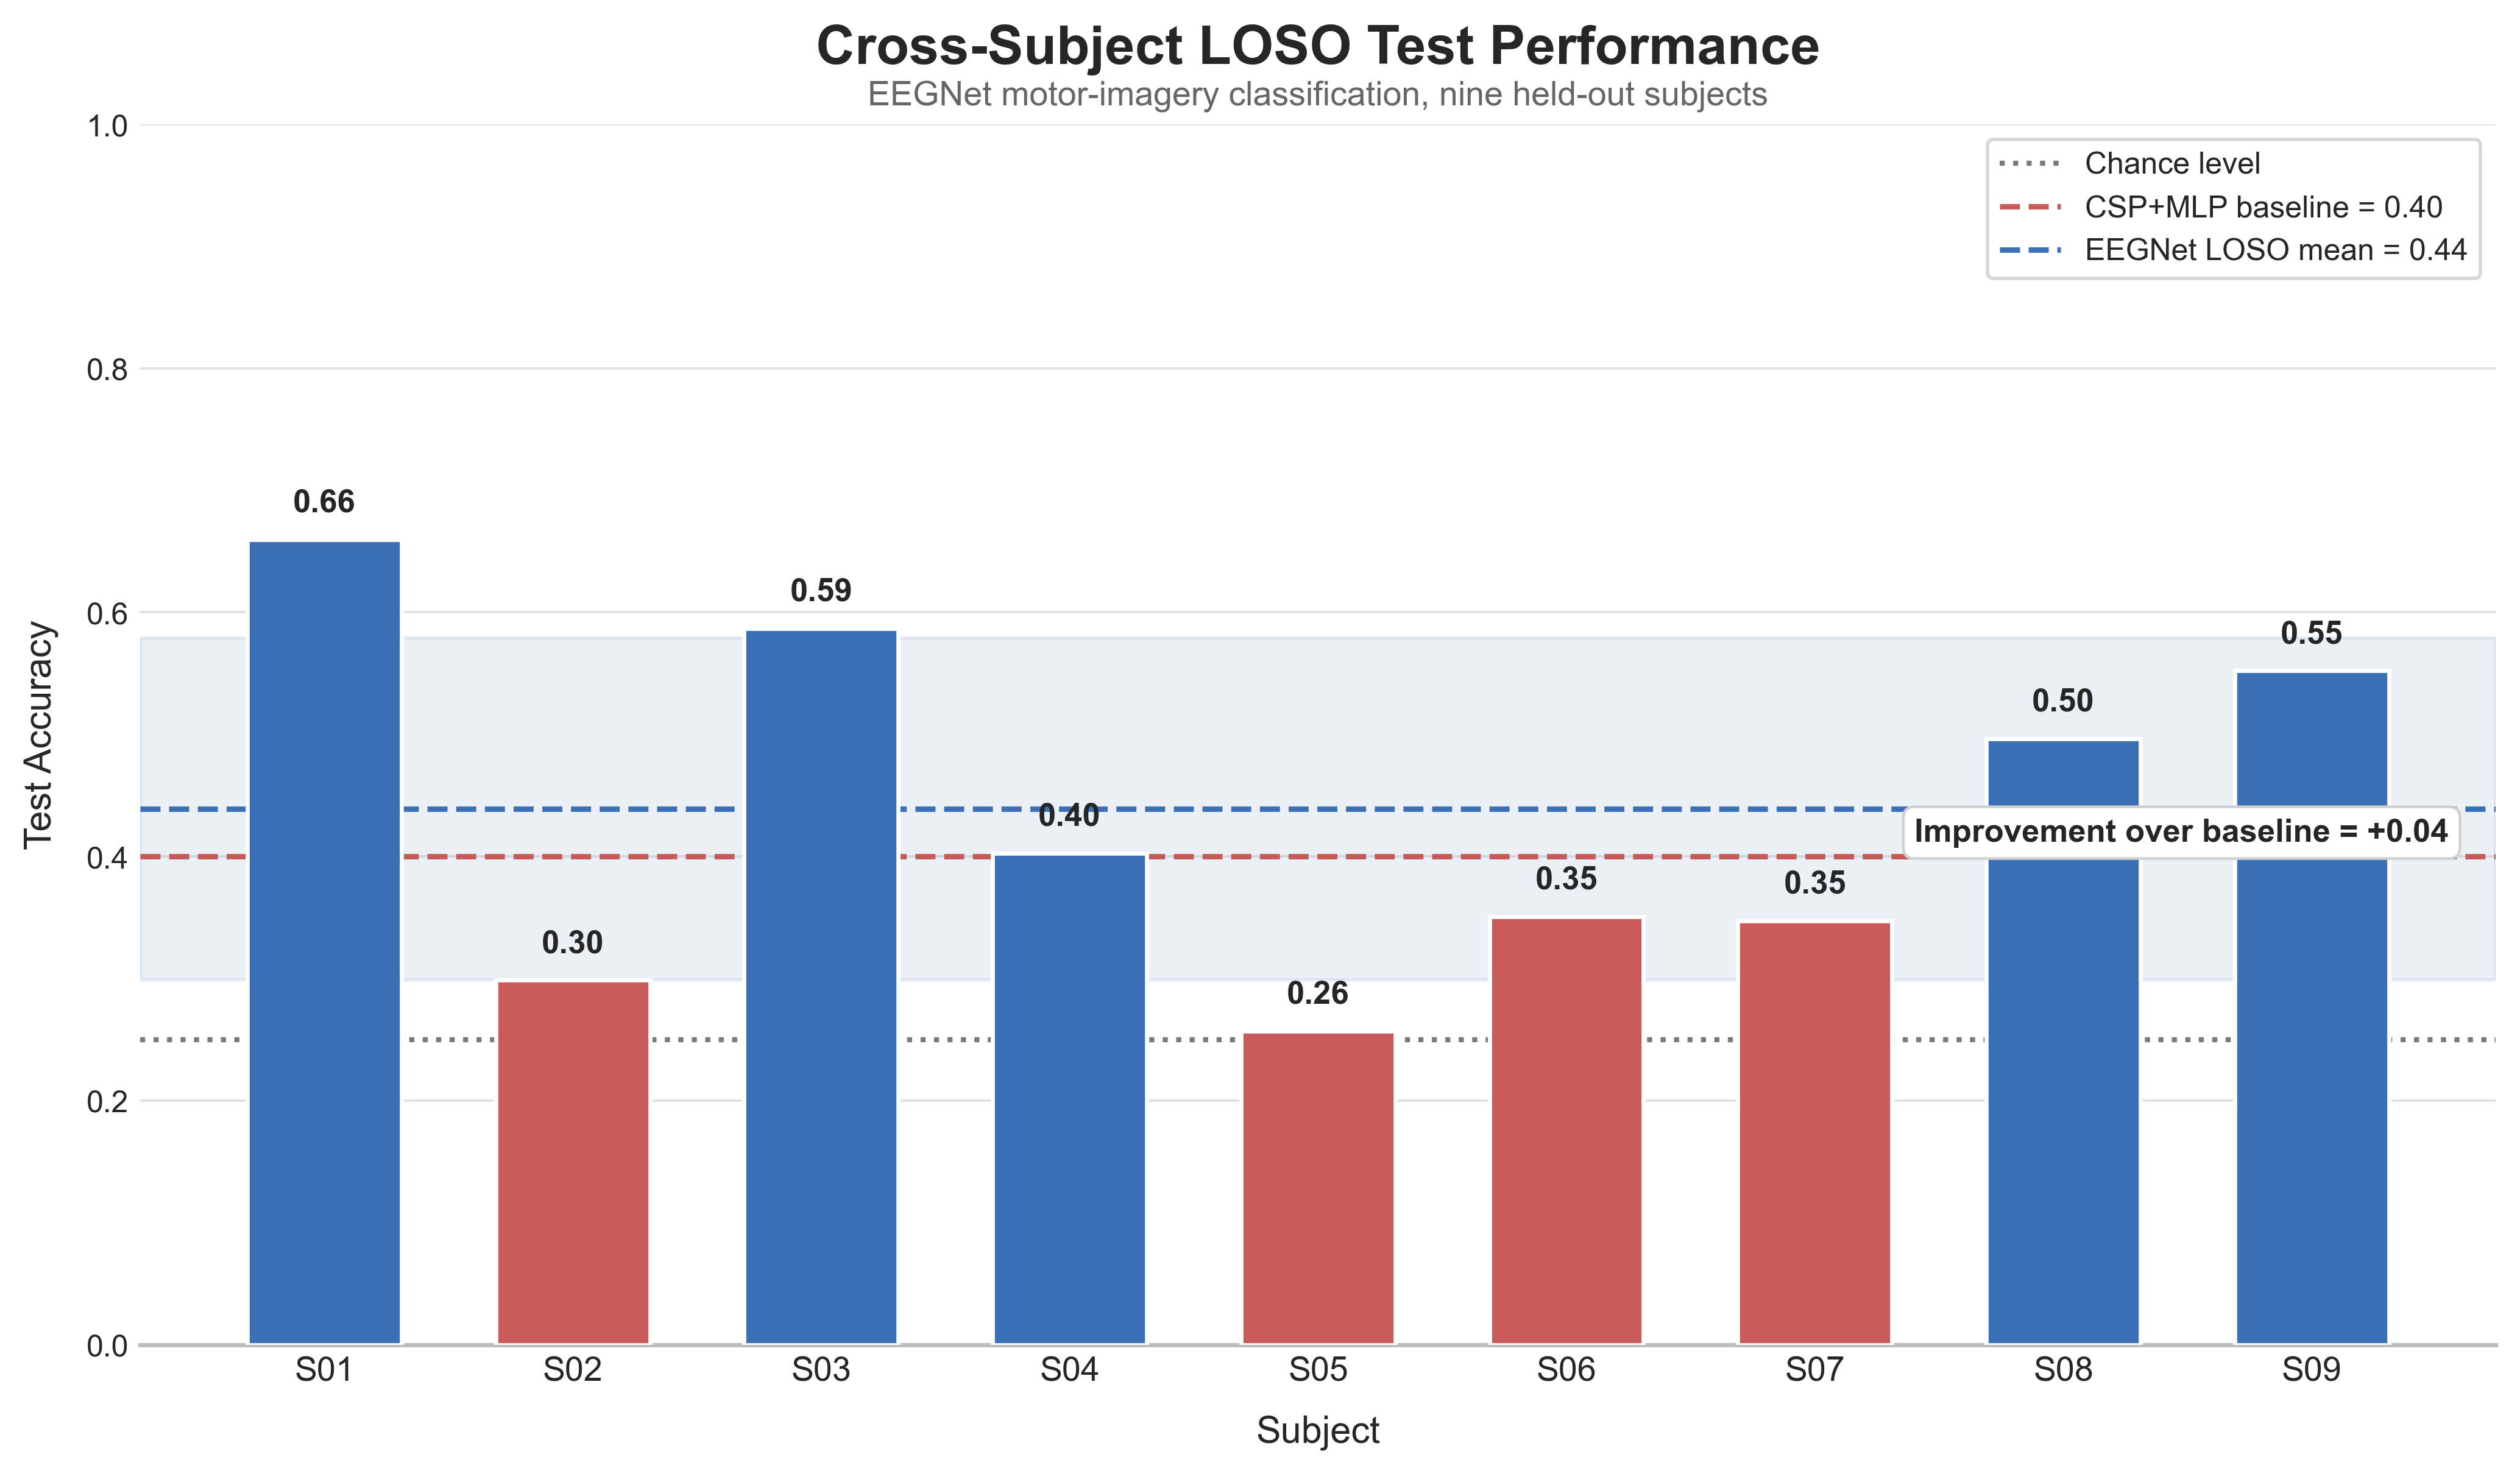
\includegraphics[width=0.85\linewidth]{../figures/final_loso_test_summary.png}
		\caption{LOSO test accuracy per subject for EEGNet, with reference lines for the CSP+MLP LOSO
			baseline mean ($40\%$) and chance level ($25\%$), and the overall EEGNet mean $\pm 1$ SD band.}
		\label{fig:exp3-accuracy}
	\end{figure}
	
	The same easy/hard subject pattern observed in Experiment~2 persists here: Subject~S01 is the most
	decodable across both hybrid and deep-learning pipelines ($0.660$ for EEGNet vs.\ $0.566$ for the
	hybrid MLP), while Subject~S05 and Subject~S02 remain the most difficult, both near chance for both
	approaches. This consistency suggests that the difficulty is intrinsic to those subjects' recordings
	(e.g.\ weaker or noisier motor-imagery-related cortical activity, or greater susceptibility to
	artifact) rather than an artifact of either particular modelling approach. The aggregated confusion
	pattern across folds (not shown) mirrors the class-wise trends already visible in
	Table~\ref{tab:exp3-loso}: Left/Right Hand trials are decoded more reliably on average than Feet and
	Tongue trials, consistent with the stronger, more lateralized ERD typically associated with hand
	motor imagery.
	
	\subsubsection{Subject-Specific Fine-Tuning (Calibration)}
	\label{sec:results-exp3-ft}
	As a realistic deployment scenario, each LOSO-trained EEGNet model was further fine-tuned on half of
	the target (previously unseen) subject's own data (a $50\%$ calibration split) for 10 additional
	epochs at a reduced learning rate, then evaluated on the remaining $50\%$ of that subject's data. The
	zero-shot vs.\ fine-tuned accuracy for each subject is reported in the last two columns of
	Table~\ref{tab:exp3-loso}.
	
	\noindent Fine-tuning raised the mean accuracy from $0.439$ (zero-shot) to $\mathbf{0.476}$, an
	absolute improvement of $+3.7$ percentage points from only $144$ calibration trials per subject
	(half of one subject's recording). Every subject improved or matched its zero-shot performance under
	fine-tuning (e.g.\ S06 improved from $0.351$ to $0.424$; S08 from $0.497$ to $0.569$), with only
	Subject~S05 showing no change, consistent with that subject's data appearing to carry very little
	class-discriminative motor-imagery signal under either pipeline. This result directly demonstrates
	that a brief, low-cost calibration phase is a practical and effective strategy for narrowing the
	cross-subject domain-shift gap in deployed BCIs.
	
	\subsection{Comparative Analysis Across All Three Experiments}
	\label{sec:comparative}
	
	\begin{table}[H]
		\centering
		\caption{Summary comparison of cross-subject / LOSO mean accuracy across all experimental
			approaches.}
		\label{tab:overall-comparison}
		\resizebox{\linewidth}{!}{%
			\begin{tabular}{lccc}
				\toprule
				\textbf{Approach} & \textbf{Mean Accuracy} & \textbf{Macro F1 / $\kappa$} & \textbf{Validation Scheme} \\
				\midrule
				Exp.\ 1: Subject-dependent (in-sample, A01T) & 0.759 & F1 = 0.760 & Single-subject held-out split \\
				Exp.\ 1: Subject-dependent (unseen, A02T--A09T) & 0.317 $\pm$ 0.074 & F1 = 0.218 & Zero-calibration transfer \\
				Exp.\ 2: LOSO, CSP+LogReg baseline & 0.382 $\pm$ 0.103 & -- & LOSO (9-fold) \\
				Exp.\ 2: LOSO, Hybrid WPD-CSP-MLP & 0.401 $\pm$ 0.125 & F1 = 0.347 & LOSO (9-fold) \\
				Exp.\ 3: LOSO, EEGNet (zero-shot) & \textbf{0.439 $\pm$ 0.140} & $\kappa$ = 0.252 & LOSO (9-fold) \\
				Exp.\ 3: LOSO, EEGNet (fine-tuned) & \textbf{0.476} & -- & LOSO + 50\% calibration \\
				\midrule
				Chance level (4 balanced classes) & 0.250 & -- & -- \\
				\bottomrule
			\end{tabular}%
		}
	\end{table}
	
	The results in Table~\ref{tab:overall-comparison} tell a
	consistent, monotonic story: (i) naive single-subject training generalizes worst
	($0.317$); (ii) pooling all subjects via LOSO cross-validation with the \emph{same} hand-engineered
	feature pipeline recovers a modest but real improvement ($0.401$); and (iii) replacing hand-engineered
	features with an end-to-end learned representation (EEGNet), evaluated under the identical LOSO
	protocol, yields the best cross-subject performance of all ($0.439$), which is further improved by a
	brief per-subject calibration step ($0.476$) -- and this is despite EEGNet operating under a
	significantly constrained training budget, as discussed next.
	
	% ============================================================
	\subsection{Side-by-Side Comparison of the Three Final Per-Subject Accuracy Charts}
	\label{sec:side-by-side}
	% ============================================================
	
	Each of the three notebooks concludes with its own summary chart plotting per-subject accuracy
	across all nine subjects. Figure~\ref{fig:three-final-charts} places these three charts side by side,
	in the same horizontal row, with a short explanation directly underneath each one.
	
	\begin{figure}[H]
		\centering
		\begin{minipage}[t]{0.32\linewidth}
			\centering
			\includegraphics[width=\linewidth]{../figures/overall_generalization_summary.png}\\[0.25cm]
			{\small\textbf{(a) Experiment 1 -- Subject-Dependent}}\\[0.15cm]
			{\footnotesize
				Naive pipeline trained on Subject~A01T only, then tested on all nine subjects. A01T (in-sample)
				scores $0.759$; the eight unseen subjects average $0.317 \pm 0.074$. Best unseen: A03T ($0.431$).
				Worst: A06T and A09T (tied, $0.253$, at chance).
			}
		\end{minipage}
		\hfill
		\begin{minipage}[t]{0.32\linewidth}
			\centering
			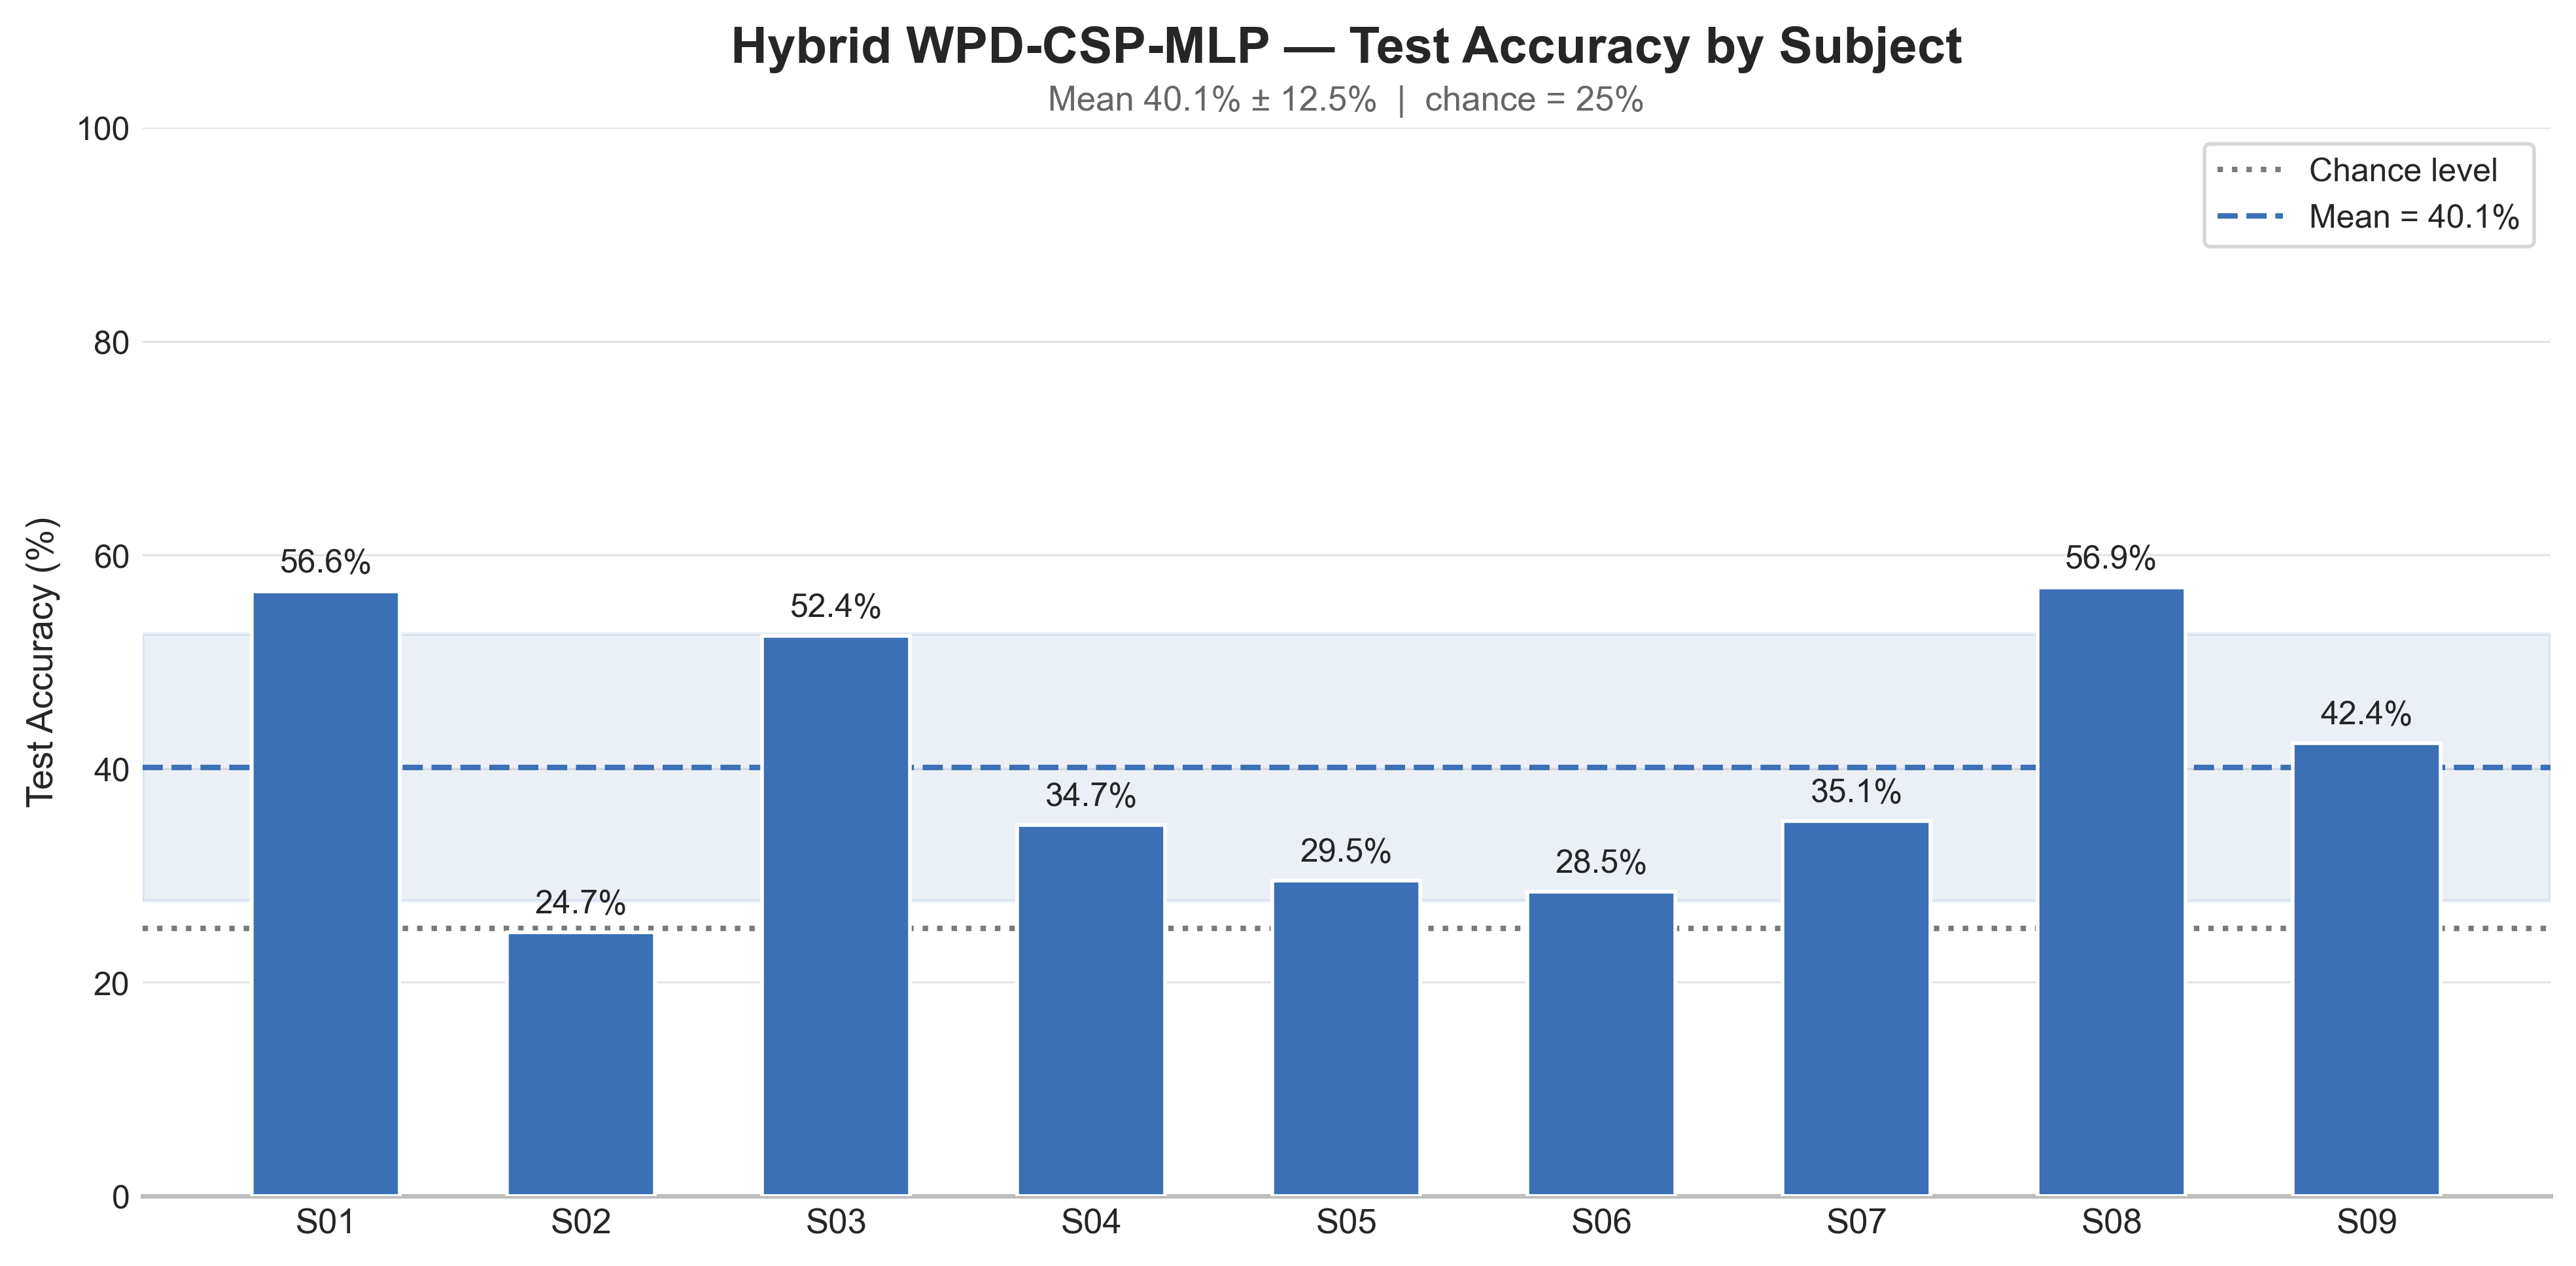
\includegraphics[width=\linewidth]{../figures/subject_accuracy_percent_mean_only.png}\\[0.25cm]
			{\small\textbf{(b) Experiment 2 -- LOSO Hybrid WPD-CSP-MLP}}\\[0.15cm]
			{\footnotesize
				Leave-One-Subject-Out accuracy for the hand-engineered WPD+CSP+MLP pipeline, all nine subjects
				now pooled during training. Mean accuracy $0.401 \pm 0.125$. Best: S08 ($0.569$), closely followed
				by S01 ($0.566$). Worst: S02 ($0.247$, at chance).
			}
		\end{minipage}
		\hfill
		\begin{minipage}[t]{0.32\linewidth}
			\centering
			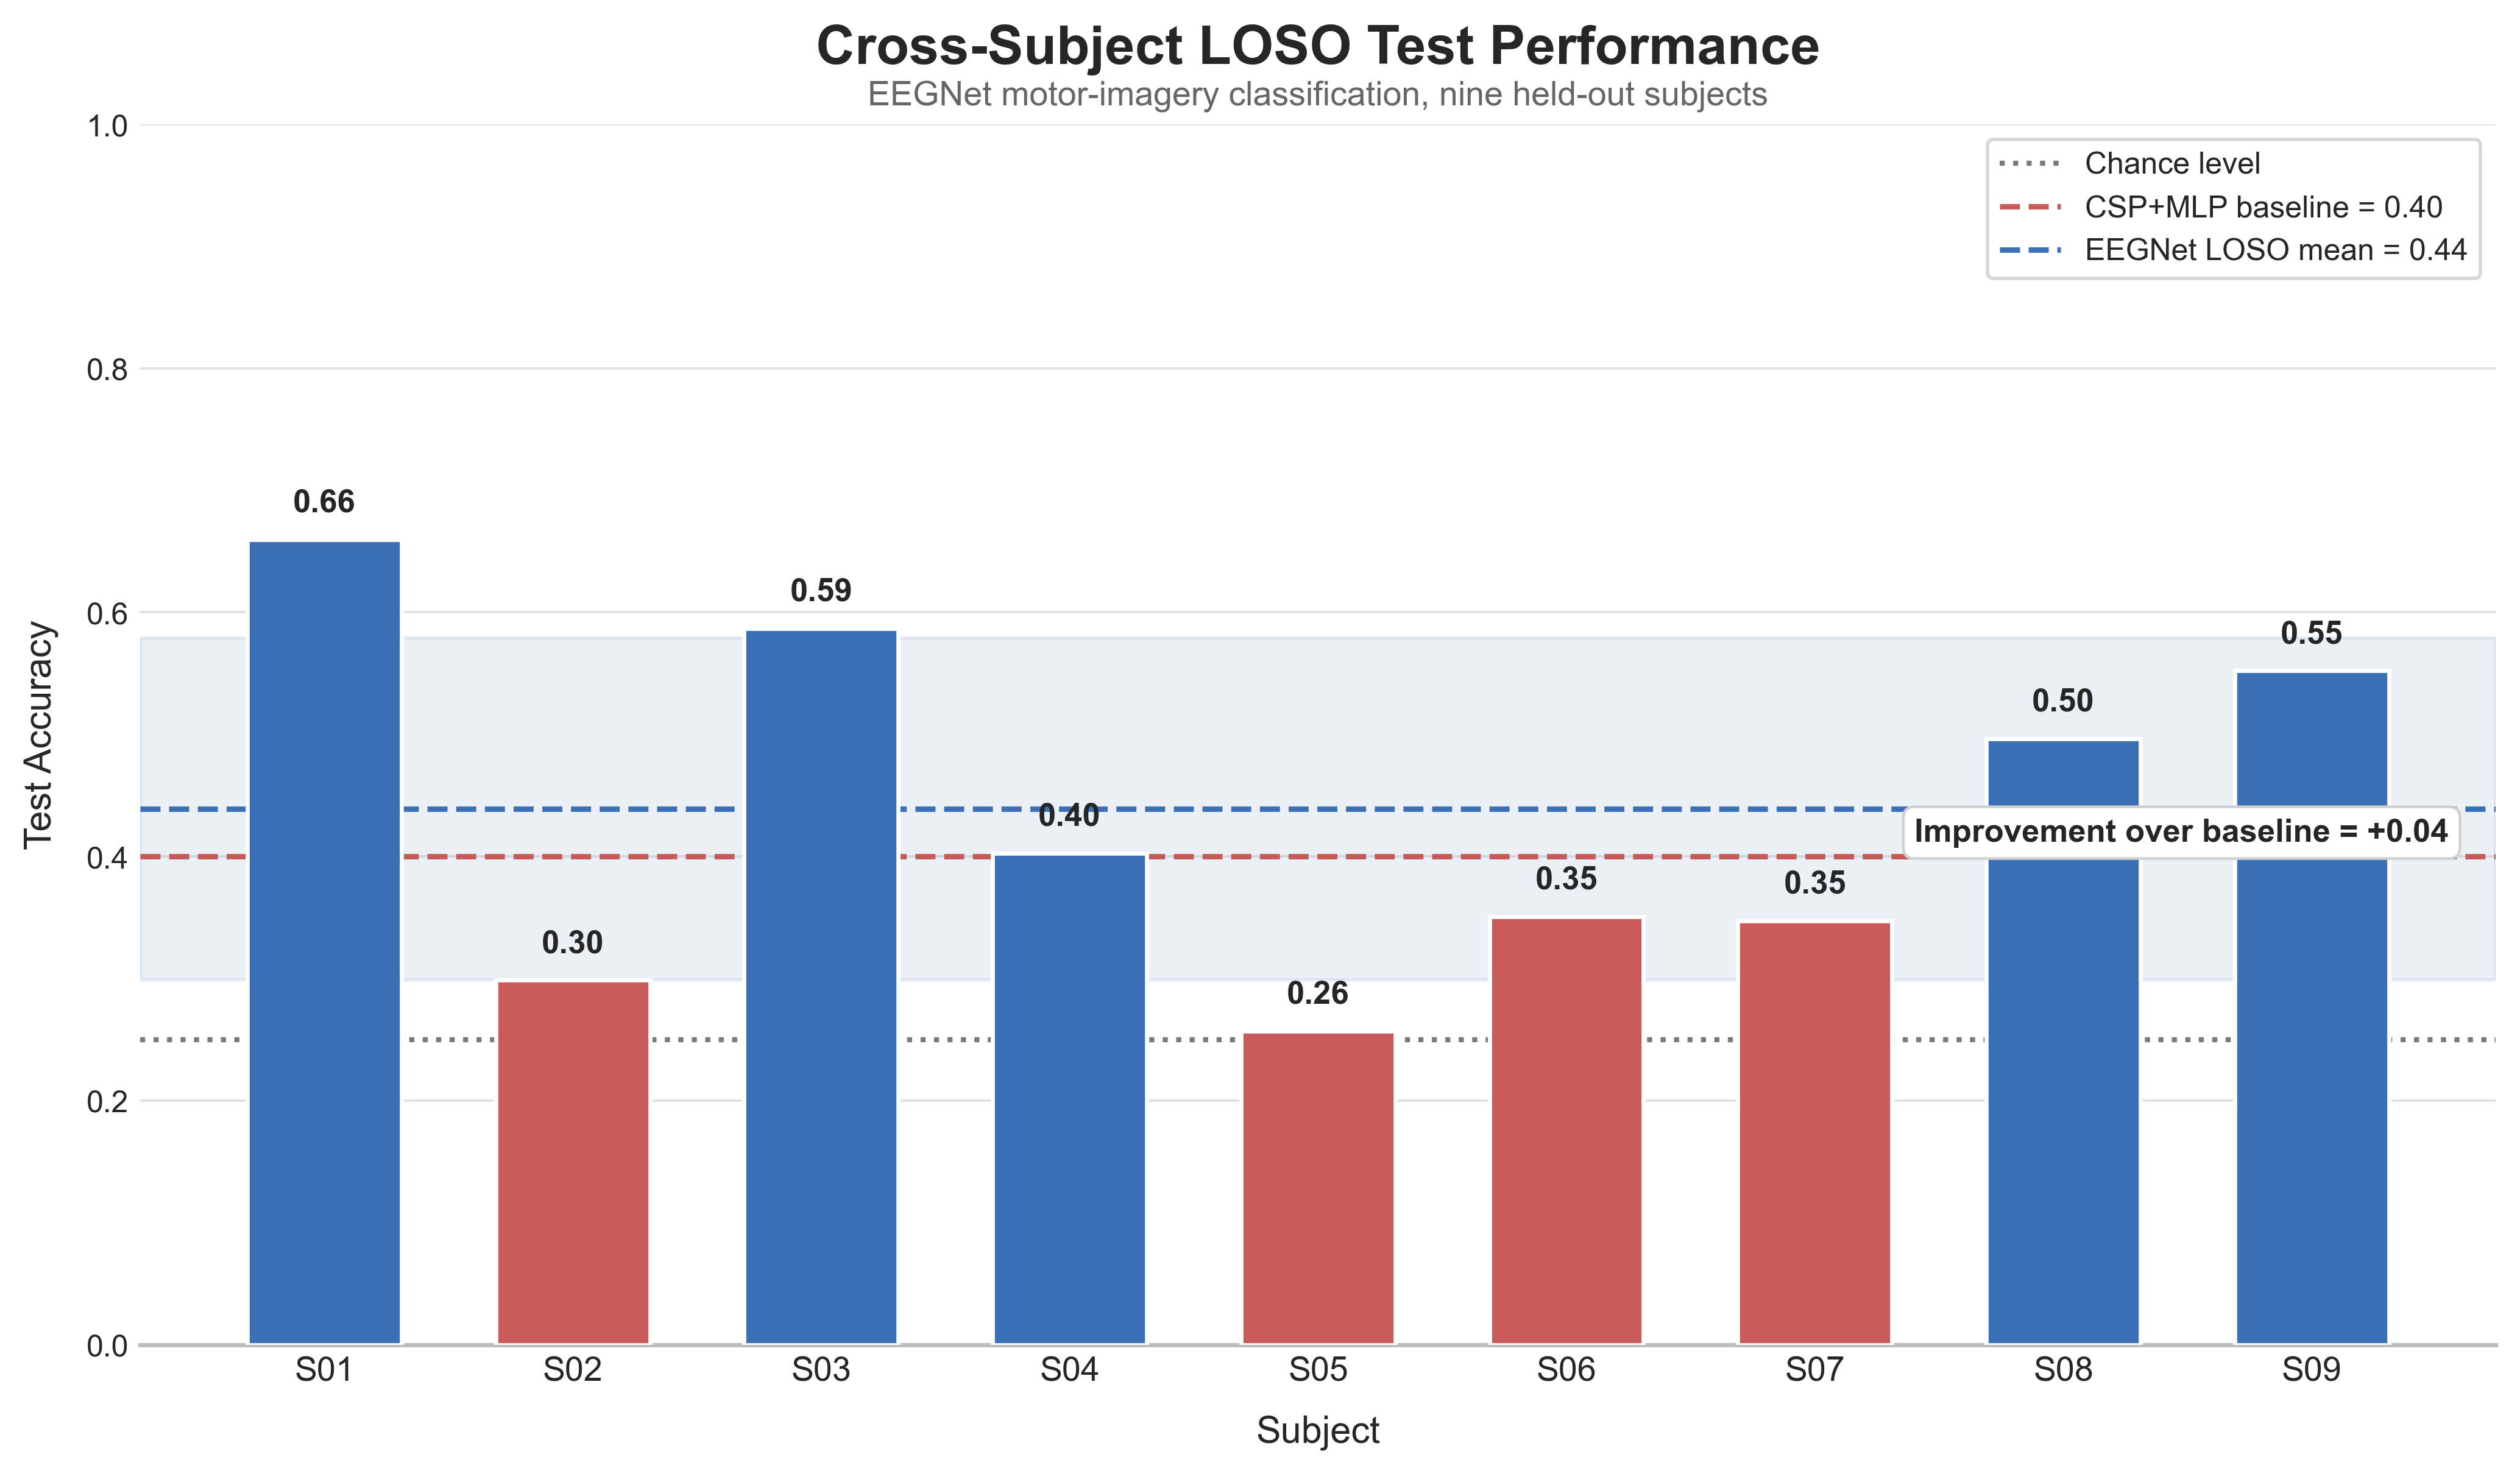
\includegraphics[width=\linewidth]{../figures/final_loso_test_summary.png}\\[0.25cm]
			{\small\textbf{(c) Experiment 3 -- LOSO EEGNet}}\\[0.15cm]
			{\footnotesize
				Leave-One-Subject-Out accuracy for the end-to-end EEGNet classifier, same protocol as (b) but with
				learned rather than hand-engineered features. Mean accuracy $0.439 \pm 0.140$ ($\kappa = 0.252$).
				Best: S01 ($0.660$). Worst: S05 ($0.257$, at chance), with S02 close behind ($0.299$).
			}
		\end{minipage}
		\caption{The three end-of-notebook per-subject accuracy summary charts, arranged side by side, with
			a brief explanation directly beneath each: (a) the naive single-subject-trained pipeline, (b) the
			LOSO Hybrid WPD-CSP-MLP classifier, and (c) the LOSO EEGNet classifier. All three plot the same nine
			subjects, allowing a direct visual comparison of both the overall accuracy level and the
			subject-to-subject pattern across approaches.}
		\label{fig:three-final-charts}
	\end{figure}
	
	\subsubsection{Overall Results}
	Read together, the three panels visually confirm the ordering already established in
	Table~\ref{tab:overall-comparison}: the bars in panel~(a) sit lowest and closest to the $0.25$
	chance line for every unseen subject, panel~(b) shows a broadly higher bar for almost every subject
	once all nine subjects are pooled during training (LOSO), and panel~(c) shows the highest bars
	overall, with several subjects (S01, S03, S09) clearing $0.55$--$0.66$ accuracy under EEGNet -- a
	level neither hand-engineered pipeline reaches for any subject except the in-sample A01T bar in
	panel~(a). The mean accuracy rises step-by-step from left to right ($0.317 \rightarrow 0.401
	\rightarrow 0.439$), and this improvement is visible as a general upward shift of the whole bar
	pattern rather than a change concentrated in one or two subjects.
	
	\subsubsection{Best- and Worst-Performing Subjects}
	Comparing \emph{across} the three panels reveals a consistent subject-level pattern that recurs
	regardless of the modelling approach used: \textbf{Subject~01} is the single most decodable
	individual in the dataset -- it achieves the highest in-sample accuracy in panel~(a) ($0.759$),
	ranks second-best in panel~(b), and is outright best in panel~(c). \textbf{Subject~03} is likewise
	consistently strong, ranking best-among-unseen in panel~(a) and top-three in both panels~(b) and~(c).
	At the other extreme, \textbf{Subject~02} is weak in every single panel ($0.316$ unseen in (a),
	$0.247$ -- the worst score -- in (b), and $0.299$ -- second-worst -- in (c)), and \textbf{Subject~05}
	is likewise persistently poor ($0.274$ in (a), $0.295$ in (b), and $0.257$ -- the worst score -- in
	(c)). Because these two subjects score near chance under three independently trained and validated
	pipelines (a hand-engineered single-subject model, a hand-engineered LOSO model, and an end-to-end
	deep network), the most plausible explanation is a genuine, subject-intrinsic limitation in the
	recorded signal quality or the strength of that individual's motor-imagery-related cortical
	response -- rather than a shortcoming specific to any one feature-extraction or classification
	method.
	
	\subsubsection{General Performance Pattern}
	A subtler pattern emerges when comparing the \emph{spread} of the bars, not just their mean height:
	the standard deviation across subjects actually \emph{increases} from panel (a) to (c) ($0.074
	\rightarrow 0.125 \rightarrow 0.140$) even as the mean improves. In other words, the accuracy gains
	achieved by moving from single-subject training, to LOSO, to EEGNet are \emph{not} shared equally by
	every subject: subjects that were already relatively decodable under the weakest pipeline (S01, S03,
	S08, S09) gain the most as stronger pipelines are introduced, while the hardest subjects (S02, S05,
	and to a lesser extent S06) remain anchored close to the $0.25$ chance line across all three charts,
	essentially unmoved by either LOSO pooling or the switch to EEGNet. This visually reinforces the
	conclusion drawn from the pairwise-transfer analysis (Section~\ref{sec:results-exp2},
	Figure~\ref{fig:pairwise-transfer}): part of the cross-subject accuracy gap in this dataset reflects
	genuine, hard-to-close differences in signal quality between individuals, rather than a limitation
	that better feature engineering or a better classifier alone can fully resolve.
	
	% ============================================================
	\section{Discussion}
	\label{sec:discussion}
	% ============================================================
	
	\subsection{Domain Shift Across Subjects}
	The pairwise transfer-accuracy heatmap (Figure~\ref{fig:pairwise-transfer}) provides the clearest
	quantitative picture of the inter-subject domain-shift problem in this dataset: within-subject
	decoding accuracy ($0.656$ mean) is more than two-and-a-half times higher than direct,
	unadapted cross-subject transfer accuracy ($0.254$ mean, statistically at chance). This gap arises
	because CSP spatial filters are, by construction, optimized to the specific spatial covariance
	structure of the class-conditional signal for the subject on which they were fit; that covariance
	structure is shaped by individual factors -- skull/scalp conductivity, cortical folding, exact
	electrode positioning relative to the sensorimotor strip, and the subject's own cognitive strategy for
	performing motor imagery -- none of which are shared across individuals. The WPD statistical features
	suffer a related, if somewhat less severe, problem: the concentration of signal energy across
	frequency sub-bands (e.g.\ where in the mu/beta range a given subject's ERD is strongest) is itself
	subject-dependent.
	
	\subsection{Why LOSO Training Helps, But Only Modestly}
	Pooling eight subjects' data before fitting CSP and the MLP (Experiment~2) forces the spatial filters
	and classifier decision boundaries to compromise across a range of individual covariance structures
	rather than over-fitting to just one. This explains the improvement from $0.317$ (single-subject
	training, tested on unseen subjects) to $0.401$ (LOSO). However, the improvement is modest because
	averaging over eight heterogeneous individual covariance structures does not produce spatial filters
	that are well-matched to \emph{any} of them in particular -- it is a compromise solution, not an
	adapted one. This is consistent with the broader finding in the BCI transfer-learning literature that
	naive data pooling recovers only part of the gap closed by explicit domain-adaptation techniques (such
	as the Euclidean Alignment already applied here, or more sophisticated Riemannian-geometry methods).
	
	\subsection{Why Deep Representations (EEGNet) Generalize Better}
	EEGNet's advantage over the hybrid hand-engineered pipeline, even under a curtailed training schedule,
	likely stems from several compounding factors:
	\begin{itemize}[leftmargin=1.2cm]
		\item \textbf{Wider, jointly-learned filter bank.} EEGNet's temporal convolution learns a bank of
		$F_1=8$ frequency-selective filters directly from the $4$--$38$\,Hz data, rather than relying on a
		single, manually-chosen $8$--$30$\,Hz band -- it can allocate representational capacity to
		whichever frequency ranges are most discriminative for the pooled training population, rather than
		a range chosen \emph{a priori} from domain knowledge.
		\item \textbf{End-to-end joint optimization.} The temporal and spatial filters in EEGNet are
		learned jointly with the classifier under a single loss function, whereas the hybrid pipeline
		fits WPD, CSP, and the MLP in three separate, sequential, unsupervised-then-supervised stages --
		each stage can only pass along information that survived the previous, independently-optimized
		stage.
		\item \textbf{Strong built-in regularization.} The max-norm weight constraints on both the
		depthwise-convolution and dense layers act as aggressive implicit regularizers well-suited to the
		modest amount of per-subject training data available, likely improving generalization more than
		the dropout-only regularization used in the MLP.
		\item \textbf{Per-trial normalization.} Z-scoring each trial independently (rather than using a
		training-set-derived global scaler, as in the hybrid pipeline) directly removes inter-subject
		amplitude/scale differences at the input level, before any learned filtering occurs.
	\end{itemize}
	
	\subsection{Impact of the Computational Constraint on the EEGNet Results}
	The results in Section~\ref{sec:results-exp3} should be interpreted as a \textbf{conservative lower
		bound} on EEGNet's true cross-subject performance on this dataset. With only 42 epochs of budget (versus a
	recommended 300) and a correspondingly shortened early-stopping patience (6 vs.\ 30), several folds
	(e.g.\ S01, S02) had not yet plateaued in validation accuracy when the epoch budget was exhausted --
	they were not stopped early by the patience criterion, but simply ran out of allotted epochs. This
	strongly suggests that a fully-trained EEGNet, given the estimated $7{+}$ hours of additional CPU time
	that were not available for this project, would likely further widen its already-observed advantage
	over the hand-engineered baselines, consistent with published EEGNet benchmarks on BCI-IV-2a that
	typically report higher LOSO accuracies under full training budgets and (in some cases) GPU-accelerated
	data augmentation.
	
	\subsection{Limitations}
	\begin{itemize}[leftmargin=1.2cm]
		\item Only the \texttt{T} (training) session per subject was usable for EEGNet due to missing
		external label files for the \texttt{E} (evaluation) sessions, halving the amount of data
		theoretically available in the original BCI-IV-2a competition protocol.
		\item The EEGNet training budget was constrained by CPU-only compute, as discussed above; results
		for EEGNet should not yet be read as reflecting its ceiling performance on this dataset.
		\item The three experiments use two different pre-processing pipelines with different band-pass
		ranges, epoch windows, and resampling rates, which somewhat complicates a perfectly like-for-like
		comparison between the hybrid and deep-learning approaches -- however, this reflects a realistic
		comparison of complete, self-consistent competing pipelines, not an ablation of a single
		variable.
		\item With only nine subjects, per-subject accuracy estimates (and their standard deviations) are
		based on limited sample sizes; some subject-to-subject differences reported here may not be
		statistically robust to a larger cohort.
	\end{itemize}
	
	% ============================================================
	\section{Future Work}
	\label{sec:future}
	% ============================================================
	
	\begin{itemize}[leftmargin=1.2cm]
		\item \textbf{Fully-trained EEGNet.} Re-run the LOSO EEGNet experiment with the originally
		intended configuration (300 epochs, patience 30, data augmentation enabled) on GPU-accelerated
		hardware to obtain an unconstrained estimate of the architecture's ceiling performance on this
		dataset, and to properly benefit from the noise-injection and time-shift augmentation strategies
		already implemented but disabled in this run.
		\item \textbf{Transfer learning and calibration.} The fine-tuning experiment
		(Section~\ref{sec:results-exp3-ft}) already demonstrates the value of brief subject-specific
		calibration; this could be extended with few-shot / meta-learning approaches (e.g.\
		model-agnostic meta-learning) explicitly optimized to adapt quickly from very small calibration
		sets, or with domain-adversarial training that encourages subject-invariant intermediate
		representations during the main LOSO training phase itself.
		\item \textbf{Riemannian-geometry methods.} Beyond Euclidean Alignment, Riemannian tangent-space
		mapping of trial covariance matrices is a well-established family of techniques for
		cross-subject BCI transfer that could be integrated with either the hybrid CSP pipeline or as a
		pre-processing step ahead of EEGNet.
		\item \textbf{Larger and more diverse cohorts.} Validating these findings on additional
		public motor-imagery datasets (e.g.\ Physionet EEGMMI, OpenBMI) with larger subject pools would
		clarify how robust the observed generalization ordering (subject-dependent~<~LOSO
		hybrid~<~LOSO EEGNet~<~fine-tuned EEGNet) is across populations and recording protocols.
		\item \textbf{Ensembling and hybridization.} Combining the CSP/WPD hand-engineered features with
		EEGNet's learned representations (e.g.\ as parallel input streams into a joint classifier, or via
		late-fusion ensembling) may capture complementary information and further improve cross-subject
		robustness beyond either approach alone.
		\item \textbf{Using both T and E sessions.} Recovering or re-deriving the true labels for the
		evaluation (\texttt{E}) sessions would double the amount of per-subject data available for
		training and calibration, which is likely to particularly benefit the data-hungry EEGNet model.
	\end{itemize}
	
	% ============================================================
	\section{Conclusion}
	\label{sec:conclusion}
	% ============================================================
	
	This report presented a systematic, three-way comparison of cross-subject generalization strategies
	for EEG motor-imagery classification on the nine-subject BCI Competition IV-2a dataset. A
	naively-trained, single-subject hybrid WPD-CSP-MLP pipeline achieves strong in-sample accuracy
	($0.759$) but generalizes poorly to unseen subjects ($0.317 \pm 0.074$, close to chance for several
	individuals), directly quantifying the severity of inter-subject domain shift in EEG-based BCIs. A
	Leave-One-Subject-Out cross-validation protocol applied to the same feature family, augmented with
	Euclidean Alignment, recovers a modest improvement to $0.401 \pm 0.125$. Replacing the hand-engineered
	feature pipeline with EEGNet, an end-to-end deep convolutional architecture, and evaluating under the
	identical LOSO protocol, achieves the best cross-subject performance of the three approaches
	($0.439 \pm 0.140$, Cohen's $\kappa = 0.252$) despite operating under a substantially reduced training
	budget necessitated by CPU-only compute -- and this figure improves further to $0.476$ with a brief,
	practical subject-specific fine-tuning step. Taken together, these findings support two central
	conclusions relevant to the design of subject-independent BCIs: first, that naive pooling of
	multi-subject training data (LOSO) only partially addresses the inter-subject domain-shift problem
	inherent to hand-engineered spatial filters such as CSP; and second, that learned, end-to-end deep
	representations such as EEGNet -- even when computationally constrained -- transfer across subjects
	more robustly than hand-engineered features, and that inexpensive per-subject calibration remains a
	highly effective complementary strategy for closing the remaining gap.
	
	% ============================================================
	%  BIBLIOGRAPHY
	% ============================================================
	\newpage
	\begin{thebibliography}{99}
		
		\bibitem{pfurtscheller1999}
		G.~Pfurtscheller and F.~H.\ Lopes da Silva,
		``Event-related EEG/MEG synchronization and desynchronization: basic principles,''
		\emph{Clinical Neurophysiology}, vol.\ 110, no.\ 11, pp.\ 1842--1857, 1999.
		
		\bibitem{lawhern2018eegnet}
		V.~J.\ Lawhern, A.~J.\ Solon, N.~R.\ Waytowich, S.~M.\ Gordon, C.~P.\ Hung, and B.~J.\ Lance,
		``EEGNet: a compact convolutional neural network for EEG-based brain-computer interfaces,''
		\emph{Journal of Neural Engineering}, vol.\ 15, no.\ 5, p.\ 056013, 2018.
		
		\bibitem{brunner2008bci}
		C.~Brunner, R.~Leeb, G.~M{\"u}ller-Putz, A.~Schl{\"o}gl, and G.~Pfurtscheller,
		\emph{BCI Competition 2008 -- Graz Data Set A}, Institute for Knowledge Discovery, Graz University of
		Technology, 2008.
		
		\bibitem{gramfort2013mne}
		A.~Gramfort, M.~Luessi, E.~Larson, D.~A.\ Engemann, D.~Strohmeier, C.~Brodbeck, R.~Goj, M.~Jas,
		T.~Brooks, L.~Parkkonen, and M.~H{\"a}m{\"a}l{\"a}inen,
		``MEG and EEG data analysis with MNE-Python,''
		\emph{Frontiers in Neuroscience}, vol.\ 7, p.\ 267, 2013.
		
		\bibitem{ang2008fbcsp}
		K.~K.\ Ang, Z.~Y.\ Chin, H.~Zhang, and C.~Guan,
		``Filter Bank Common Spatial Pattern (FBCSP) in Brain-Computer Interface,''
		in \emph{Proc.\ IEEE International Joint Conference on Neural Networks (IJCNN)}, 2008, pp.\
		2390--2397.
		
		\bibitem{he2020ea}
		H.~He and D.~Wu,
		``Transfer learning for brain-computer interfaces: A Euclidean space data alignment approach,''
		\emph{IEEE Transactions on Biomedical Engineering}, vol.\ 67, no.\ 2, pp.\ 399--410, 2020.
		
		\bibitem{ramoser2000csp}
		H.~Ramoser, J.~M{\"u}ller-Gerking, and G.~Pfurtscheller,
		``Optimal spatial filtering of single trial EEG during imagined hand movement,''
		\emph{IEEE Transactions on Rehabilitation Engineering}, vol.\ 8, no.\ 4, pp.\ 441--446, 2000.
		
		\bibitem{cohen1960kappa}
		J.~Cohen,
		``A coefficient of agreement for nominal scales,''
		\emph{Educational and Psychological Measurement}, vol.\ 20, no.\ 1, pp.\ 37--46, 1960.
		
		\bibitem{paszke2019pytorch}
		A.~Paszke, S.~Gross, F.~Massa, A.~Lerer, J.~Bradbury, G.~Chanan, T.~Killeen, Z.~Lin, N.~Gimelshein,
		L.~Antiga, et al.,
		``PyTorch: An imperative style, high-performance deep learning library,''
		in \emph{Advances in Neural Information Processing Systems (NeurIPS)}, vol.\ 32, 2019.
		
	\end{thebibliography}
	
	% ============================================================
	%  APPENDIX
	% ============================================================
	\newpage
	\appendix
	\section{Additional Figures}
	\label{app:extra-figs}
	
	This appendix collects supplementary diagnostic figures referenced in the main text but not central
	to the primary results narrative.
	
	\subsection{Experiment 1 -- Supplementary Figures}
	
	\begin{figure}[H]
		\centering
		\includegraphics[width=0.6\linewidth]{../figures/sensor_layout.png}
		\caption{10--20 electrode layout used for Subject A01T recordings, showing the 22 EEG and 3 EOG
			sensor positions after channel renaming.}
		\label{fig:sensor-layout}
	\end{figure}
	
	\begin{figure}[H]
		\centering
		\includegraphics[width=0.85\linewidth]{../figures/ica_eog_scores.png}
		\caption{ICA component--EOG correlation scores used to automatically flag ocular-artifact
			components for removal (threshold $=2.5$), Subject A01T. Flagged components are excluded from the
			reconstructed signal prior to band-pass filtering.}
		\label{fig:ica-eog-scores}
	\end{figure}
	
	\begin{figure}[H]
		\centering
		\includegraphics[width=0.85\linewidth]{../figures/erd_sanity_check.png}
		\caption{Sanity check for event-related desynchronization (ERD): mean power spectral density at
			channels C3 and C4 for left- vs.\ right-hand imagery, Subject A01T. The expected contralateral ERD
			pattern is visible within the shaded mu+beta band.}
		\label{fig:erd-sanity}
	\end{figure}
	
	\begin{figure}[H]
		\centering
		\includegraphics[width=0.9\linewidth]{../figures/csp_topomaps.png}
		\caption{CSP spatial-filter topographies for each of the three relevant WPD sub-bands (rows) and the
			top four spatial components (columns), Subject A01T.}
		\label{fig:csp-topomaps}
	\end{figure}
	
	\begin{figure}[H]
		\centering
		\includegraphics[width=0.85\linewidth]{../figures/training_curves.png}
		\caption{Training and validation loss/accuracy curves for the subject-dependent MLP (Subject A01T
			only). Early stopping halted training at epoch 65; the lowest-validation-loss weights were restored.}
		\label{fig:exp1-training-curves}
	\end{figure}
	
	\begin{figure}[H]
		\centering
		\includegraphics[width=0.7\linewidth]{../figures/overall_generalization_summary.png}
		\caption{Overall cross-subject generalization summary: per-subject accuracy with reference lines for
			chance level, in-sample (A01T) accuracy, and mean unseen-subject accuracy; the shaded band indicates
			$\pm 1$ SD across unseen subjects.}
		\label{fig:overall-generalization-summary}
	\end{figure}
	
	\subsection{Experiment 2 -- Supplementary Figures}
	
	\begin{figure}[H]
		\centering
		\includegraphics[width=0.75\linewidth]{../figures/subject_data_summary.png}
		\caption{Per-subject trial counts by class (stacked bars) and number of ICA components removed as
			ocular artifacts (line), across all nine subjects.}
		\label{fig:subject-data-summary}
	\end{figure}
	
	\begin{figure}[H]
		\centering
		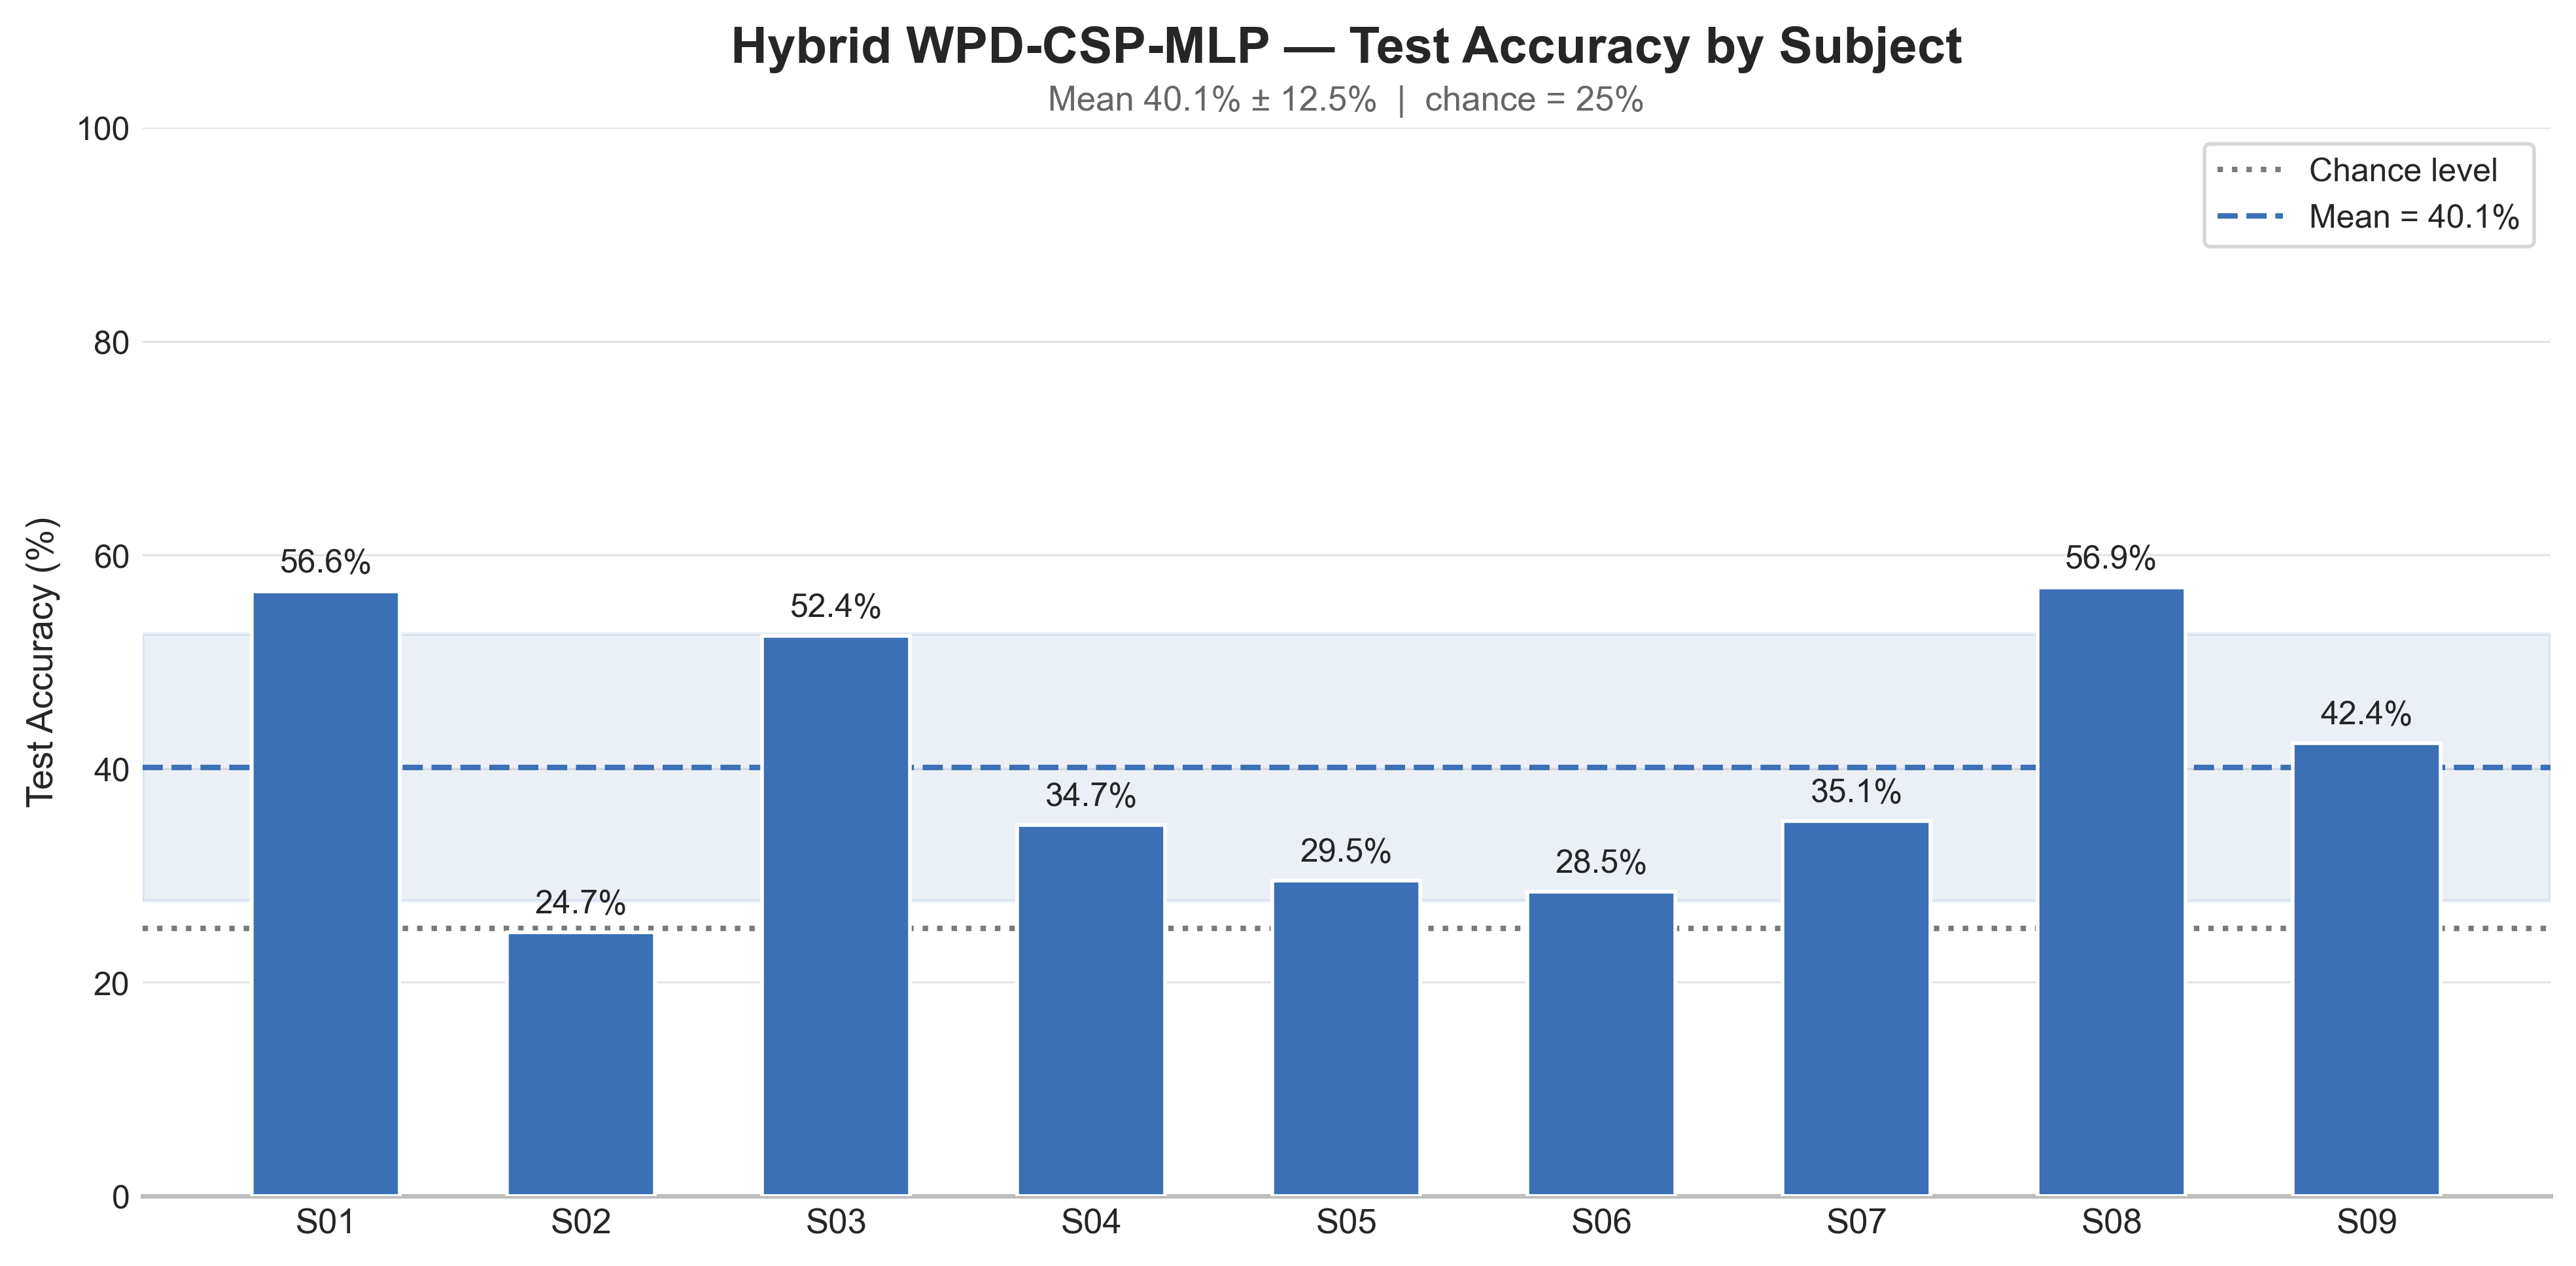
\includegraphics[width=0.7\linewidth]{../figures/subject_accuracy_percent_mean_only.png}
		\caption{Simplified per-subject mean-accuracy summary for the LOSO Hybrid WPD-CSP-MLP classifier,
			expressed as a percentage, without the baseline or per-class breakdown shown in
			Figure~\ref{fig:exp2-accuracy}.}
		\label{fig:exp2-f1-spread}
	\end{figure}
	
	\begin{table}[H]
		\centering
		\caption{Experiment 2 -- full per-class F1-score breakdown across all nine LOSO folds.}
		\label{tab:exp2-perclass-full}
		\begin{tabular}{lcccc}
			\toprule
			\textbf{Test Subject} & \textbf{F1 (Left Hand)} & \textbf{F1 (Right Hand)} & \textbf{F1 (Feet)} & \textbf{F1 (Tongue)} \\
			\midrule
			S01 & 0.634 & 0.680 & 0.581 & 0.150 \\
			S02 & 0.000 & 0.218 & 0.382 & 0.027 \\
			S03 & 0.576 & 0.442 & 0.465 & 0.532 \\
			S04 & 0.286 & 0.419 & 0.026 & 0.443 \\
			S05 & 0.345 & 0.388 & 0.182 & 0.000 \\
			S06 & 0.053 & 0.000 & 0.225 & 0.453 \\
			S07 & 0.438 & 0.454 & 0.301 & 0.000 \\
			S08 & 0.528 & 0.639 & 0.548 & 0.556 \\
			S09 & 0.482 & 0.396 & 0.140 & 0.500 \\
			\bottomrule
		\end{tabular}
	\end{table}
	
	\begin{figure}[H]
		\centering
		\includegraphics[width=0.9\linewidth]{../figures/confusion_matrix_grid.png}
		\caption{Per-subject confusion matrices for all nine LOSO folds (Hybrid WPD-CSP-MLP).}
		\label{fig:exp2-cm-grid}
	\end{figure}
	
	\begin{figure}[H]
		\centering
		\includegraphics[width=0.85\linewidth]{../figures/training_curves_all_folds.png}
		\caption{Validation loss and accuracy trajectories for the MLP across all nine LOSO folds,
			illustrating training stability across subjects.}
		\label{fig:exp2-training-all}
	\end{figure}
	
	\begin{figure}[H]
		\centering
		\includegraphics[width=0.95\linewidth]{../figures/csp_topomap_across_subjects.png}
		\caption{CSP component 0 topography (first relevant sub-band) fitted independently for each subject,
			illustrating inter-subject variability in the optimal spatial filter -- a visual counterpart to the
			domain-shift result of Figure~\ref{fig:pairwise-transfer}.}
		\label{fig:csp-across-subjects}
	\end{figure}
	
	\begin{figure}[H]
		\centering
		\includegraphics[width=0.85\linewidth]{../figures/wpd_energy_by_subject.png}
		\caption{WPD energy feature distribution (sensorimotor ROI average, pooled sub-bands) by subject and
			class, illustrating heterogeneous energy scales across subjects.}
		\label{fig:wpd-energy-by-subject}
	\end{figure}
	
	\begin{figure}[H]
		\centering
		\includegraphics[width=0.9\linewidth]{../figures/comprehensive_summary_dashboard.png}
		\caption{Consolidated LOSO results dashboard summarizing per-subject Hybrid-MLP vs.\ baseline
			accuracy alongside auxiliary summary statistics.}
		\label{fig:comprehensive-dashboard}
	\end{figure}
	
\end{document}